\section{Experiments}
\label{sec:exp}
\subsection{Implementation details}
We utilized a simple and lightweight CNN for two reasons. The first is to demonstrate the effectiveness of the proposed method without depending on the complex network structure. The second reason pertains to the nature of the training process, which involves learning from a single pair of images at a time. In the typical image restoration training, a large dataset comprising multiple pairs of degraded and ground-truth images is used. In such cases, the training network tends to be deep and complex to capture the diversity of all possible pairs in the learned weights. However, the training in our proposed method involves either a single pair or a single image, thus resulting in significantly less diversity in relationships; therefore, a relatively smaller and simpler network is sufficient. Fig.~\ref{fig:network} shows the constructed network, which comprises eight hidden layers with 64 channels each. ReLU activation is applied to each layer, and the final layer features a skip connection linked to the input layer. In the ZSSR network, the only addition to the base network is an module that upsamples the input patch by a factor of n, as shown in Fig.~\ref{fig:network}. All the experiments were conducted on an NVIDIA A100 GPU using PyTorch~\cite{paszke2019pytorch}. We optimized the parameters of the network $\mathcal{D}$ by minimizing the $L_1$ pixel loss.
\begin{equation}
    \mathcal{L} = ||\mathcal{D}(I_{source}) - I_{target}||_1,
\end{equation}
where $I_{source}$ is the source image, and $I_{target}$ is the target image. During training, the patch size was set to $96\times96$. An Adam optimizer~\cite{kingma2014adam} with $\beta_1=0.9$ and $\beta_2=0.999$ was
used to train the network for 15,000 iterations. The learning rate was initially set to $1e^{-5}$ which decayed by 10 after 10,000 iterations.

The data used for training comprised THz SAHS images measured using a THz-TDS system based on the USAF 1951 resolution test chart. For each training session, we selected two frequencies from the THz SAHS image to establish input-target mapping.

\begin{figure}[ht]
    \centering
    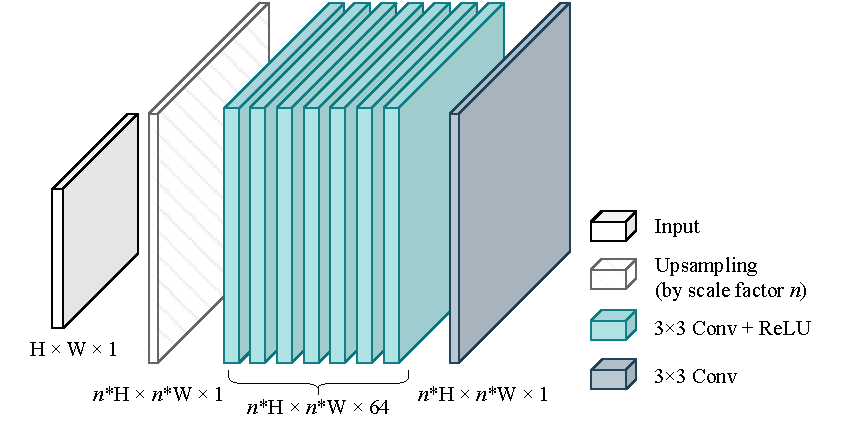
\includegraphics[width=\columnwidth]{fig/Ryu-fig8.pdf}
    \caption{Network architecture used in proposed image restoration framework. Upsampling module is used only for ZSSR training.}
    \label{fig:network}
\end{figure}

\subsection{Data Preprocessing}
To acquire THz SAHS images of the USAF 1951 resolution test chart, the THz-TDS system was used to measure time-domain pulse signals at each pixel composing the image. Each time-domain pulse signal was captured with 1000 points within a 30 ps time window, as shown in Fig.~\ref{fig:system}.
The THz-TDS imaging system employs a fast-scanning method to quickly acquire THz signals. To reduce the image acquisition time, the sample was propagated along a zigzag path and then reshaped into two dimensions based on the path. Because of the hardware limitations of the system in the zigzag scanning process, the pixels in the even and odd rows were not aligned precisely. To resolve this issue, the pixels in the odd rows were shifted by $1/5$ of a pixel to align them with those in the even rows. Additionally, areas with pixel values of 0 around the image edges were removed, i.e., only significant regions of the data were used for training. The time-domain signal data of all pixels measured via THz-TDS were converted into frequency data using the FFT to acquire SAHS images. To perform training, all the pixel intensity values were normalized to between 0 and 255. Fig.~\ref{fig:tds_freq_point} shows the time- and frequency-domain signals of the most intense THz signal pixel in the THz SAHS image, and a 2.0 THz image measuring $282\times282$ pixels. Figs.~\ref{fig:tds_freq_point}a and b show the THz time-domain signal measured at the red dot shown in the 2 THz image in Fig.~\ref{fig:tds_freq_point}c, and the corresponding frequency-domain signal obtained via FFT, respectively.

\begin{figure}[htbp]
    \centering
    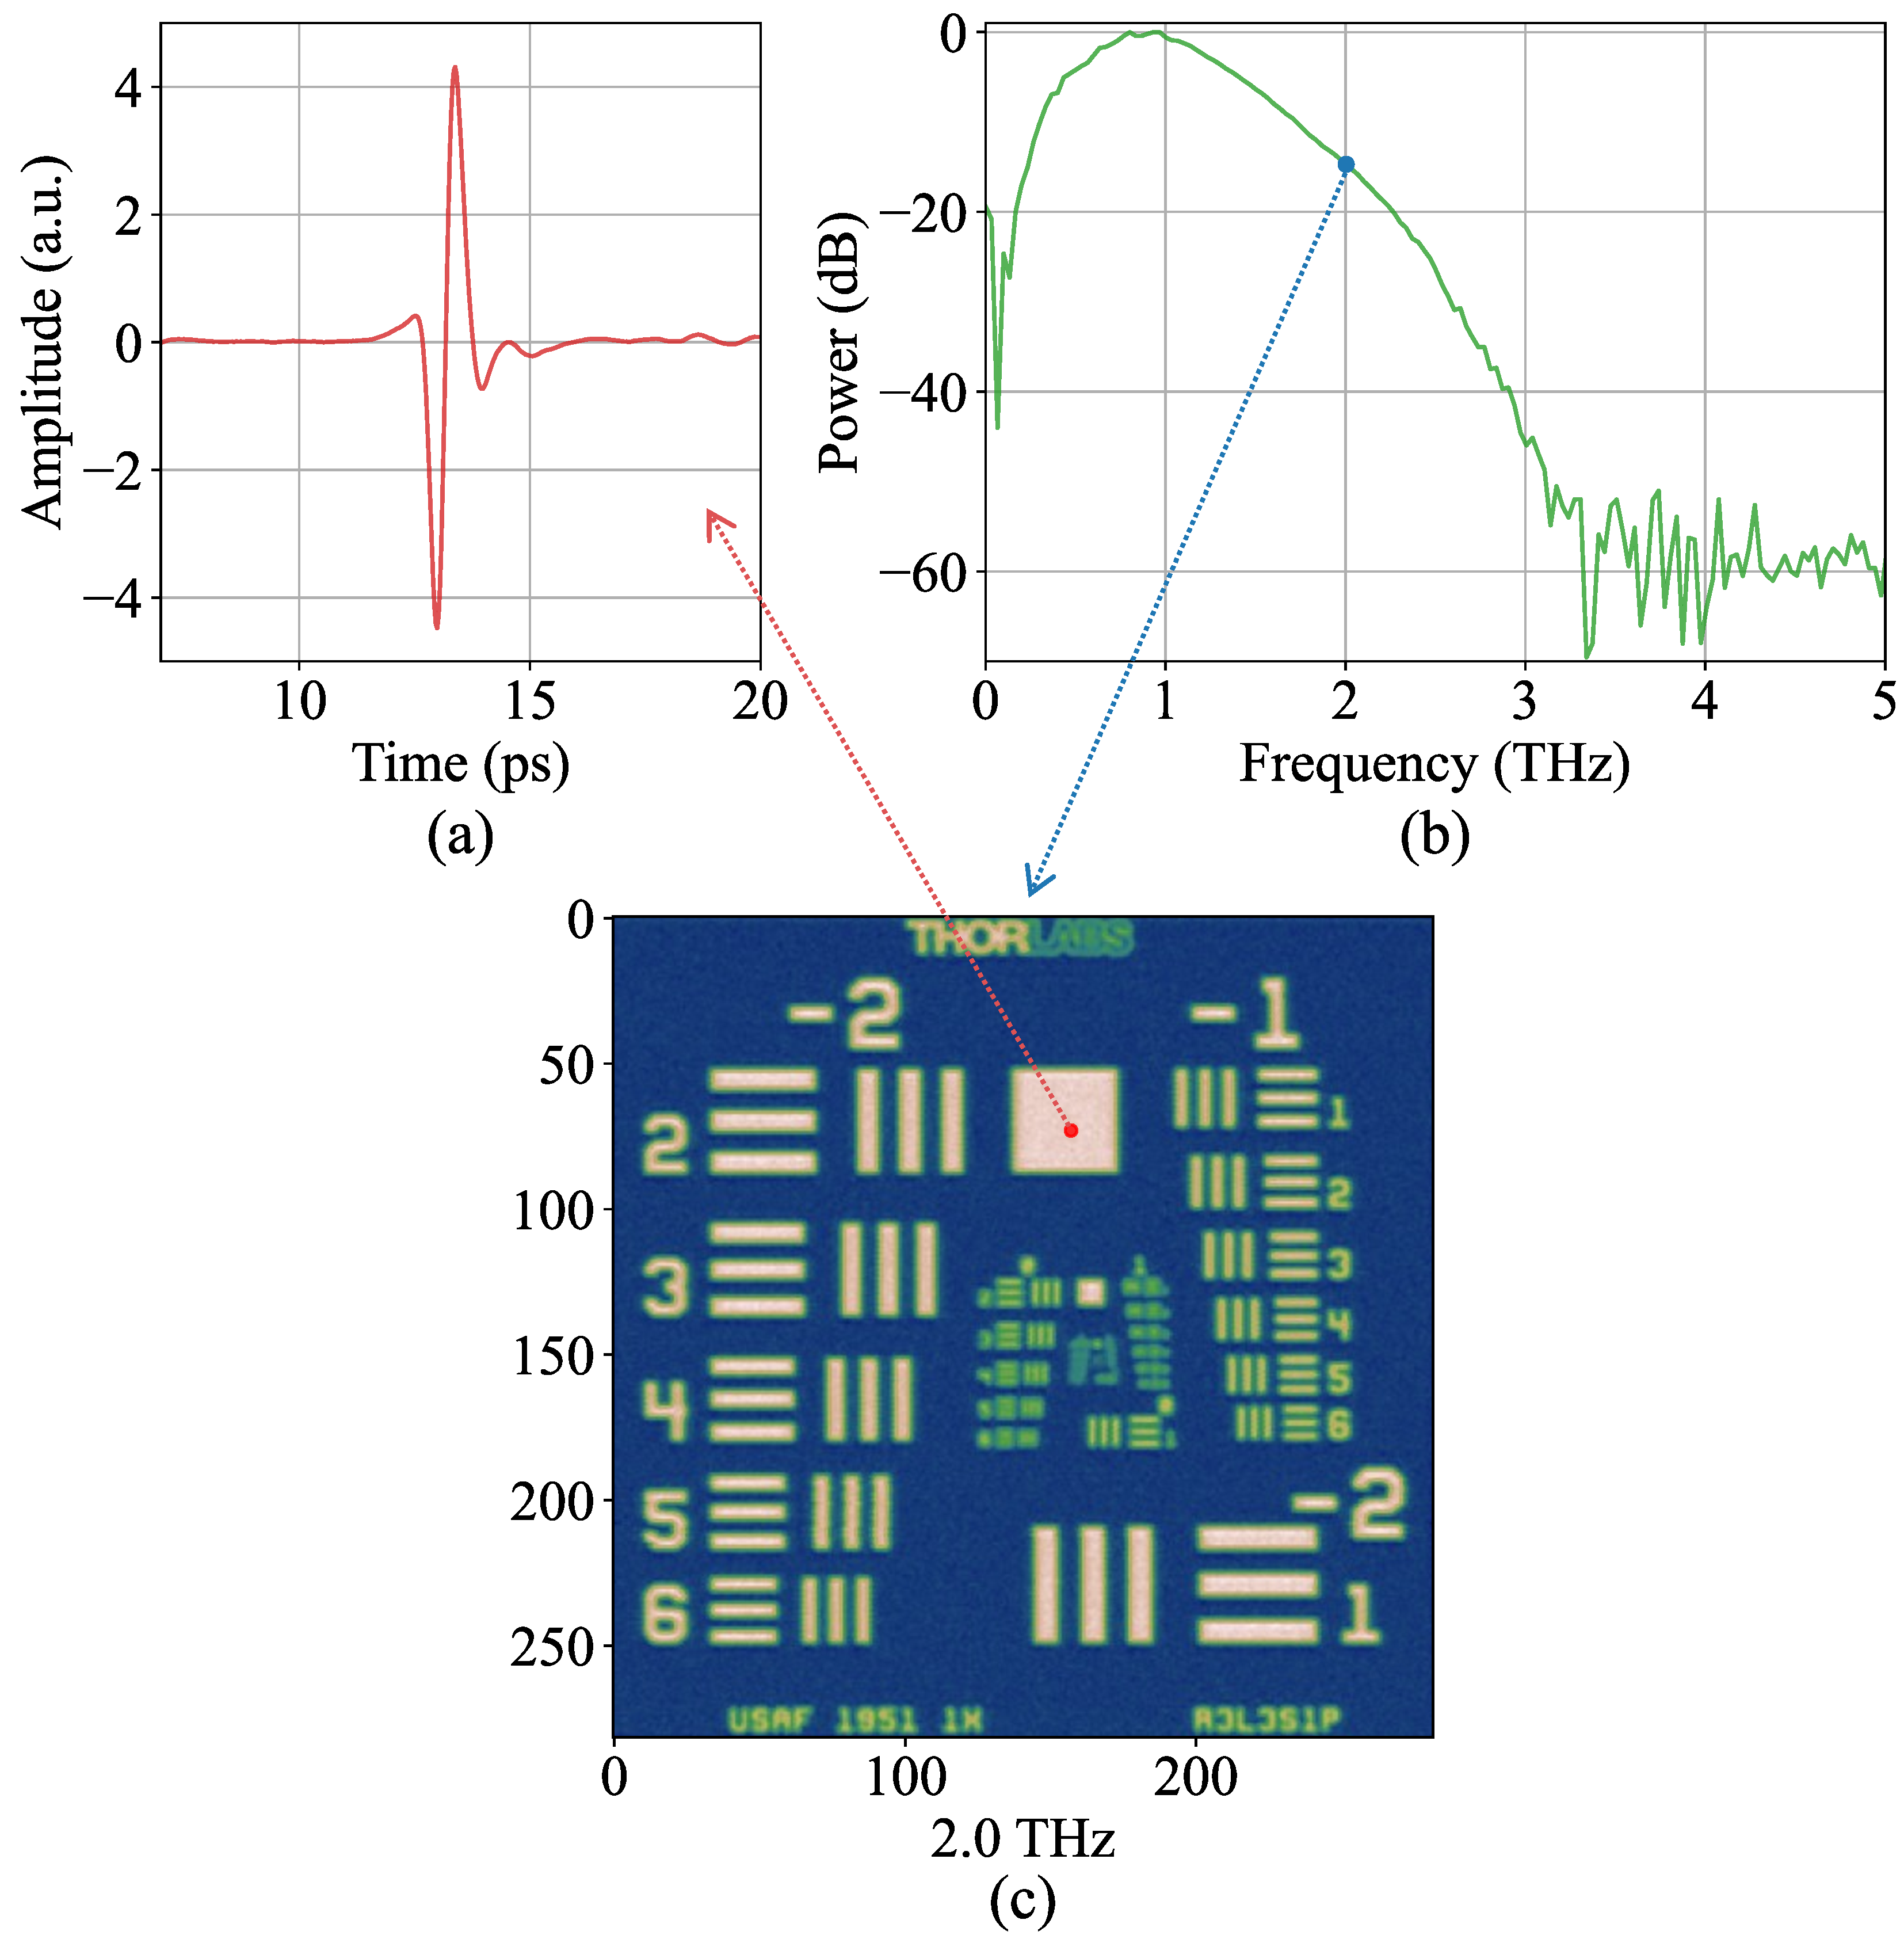
\includegraphics[width=\columnwidth]{fig/Ryu-fig9.pdf}
    \caption{Example of THz data. (a) Maximum power time-domain data (red point at (c)); (b) frequency-domain data; (c) 2.0 THz image (blue point at (b)).}
    \label{fig:tds_freq_point}
\end{figure}

\subsection{Self-Supervised Intra-Data Inference}
\label{sec:intra}
\begin{figure*}[htbp]
    \centering
    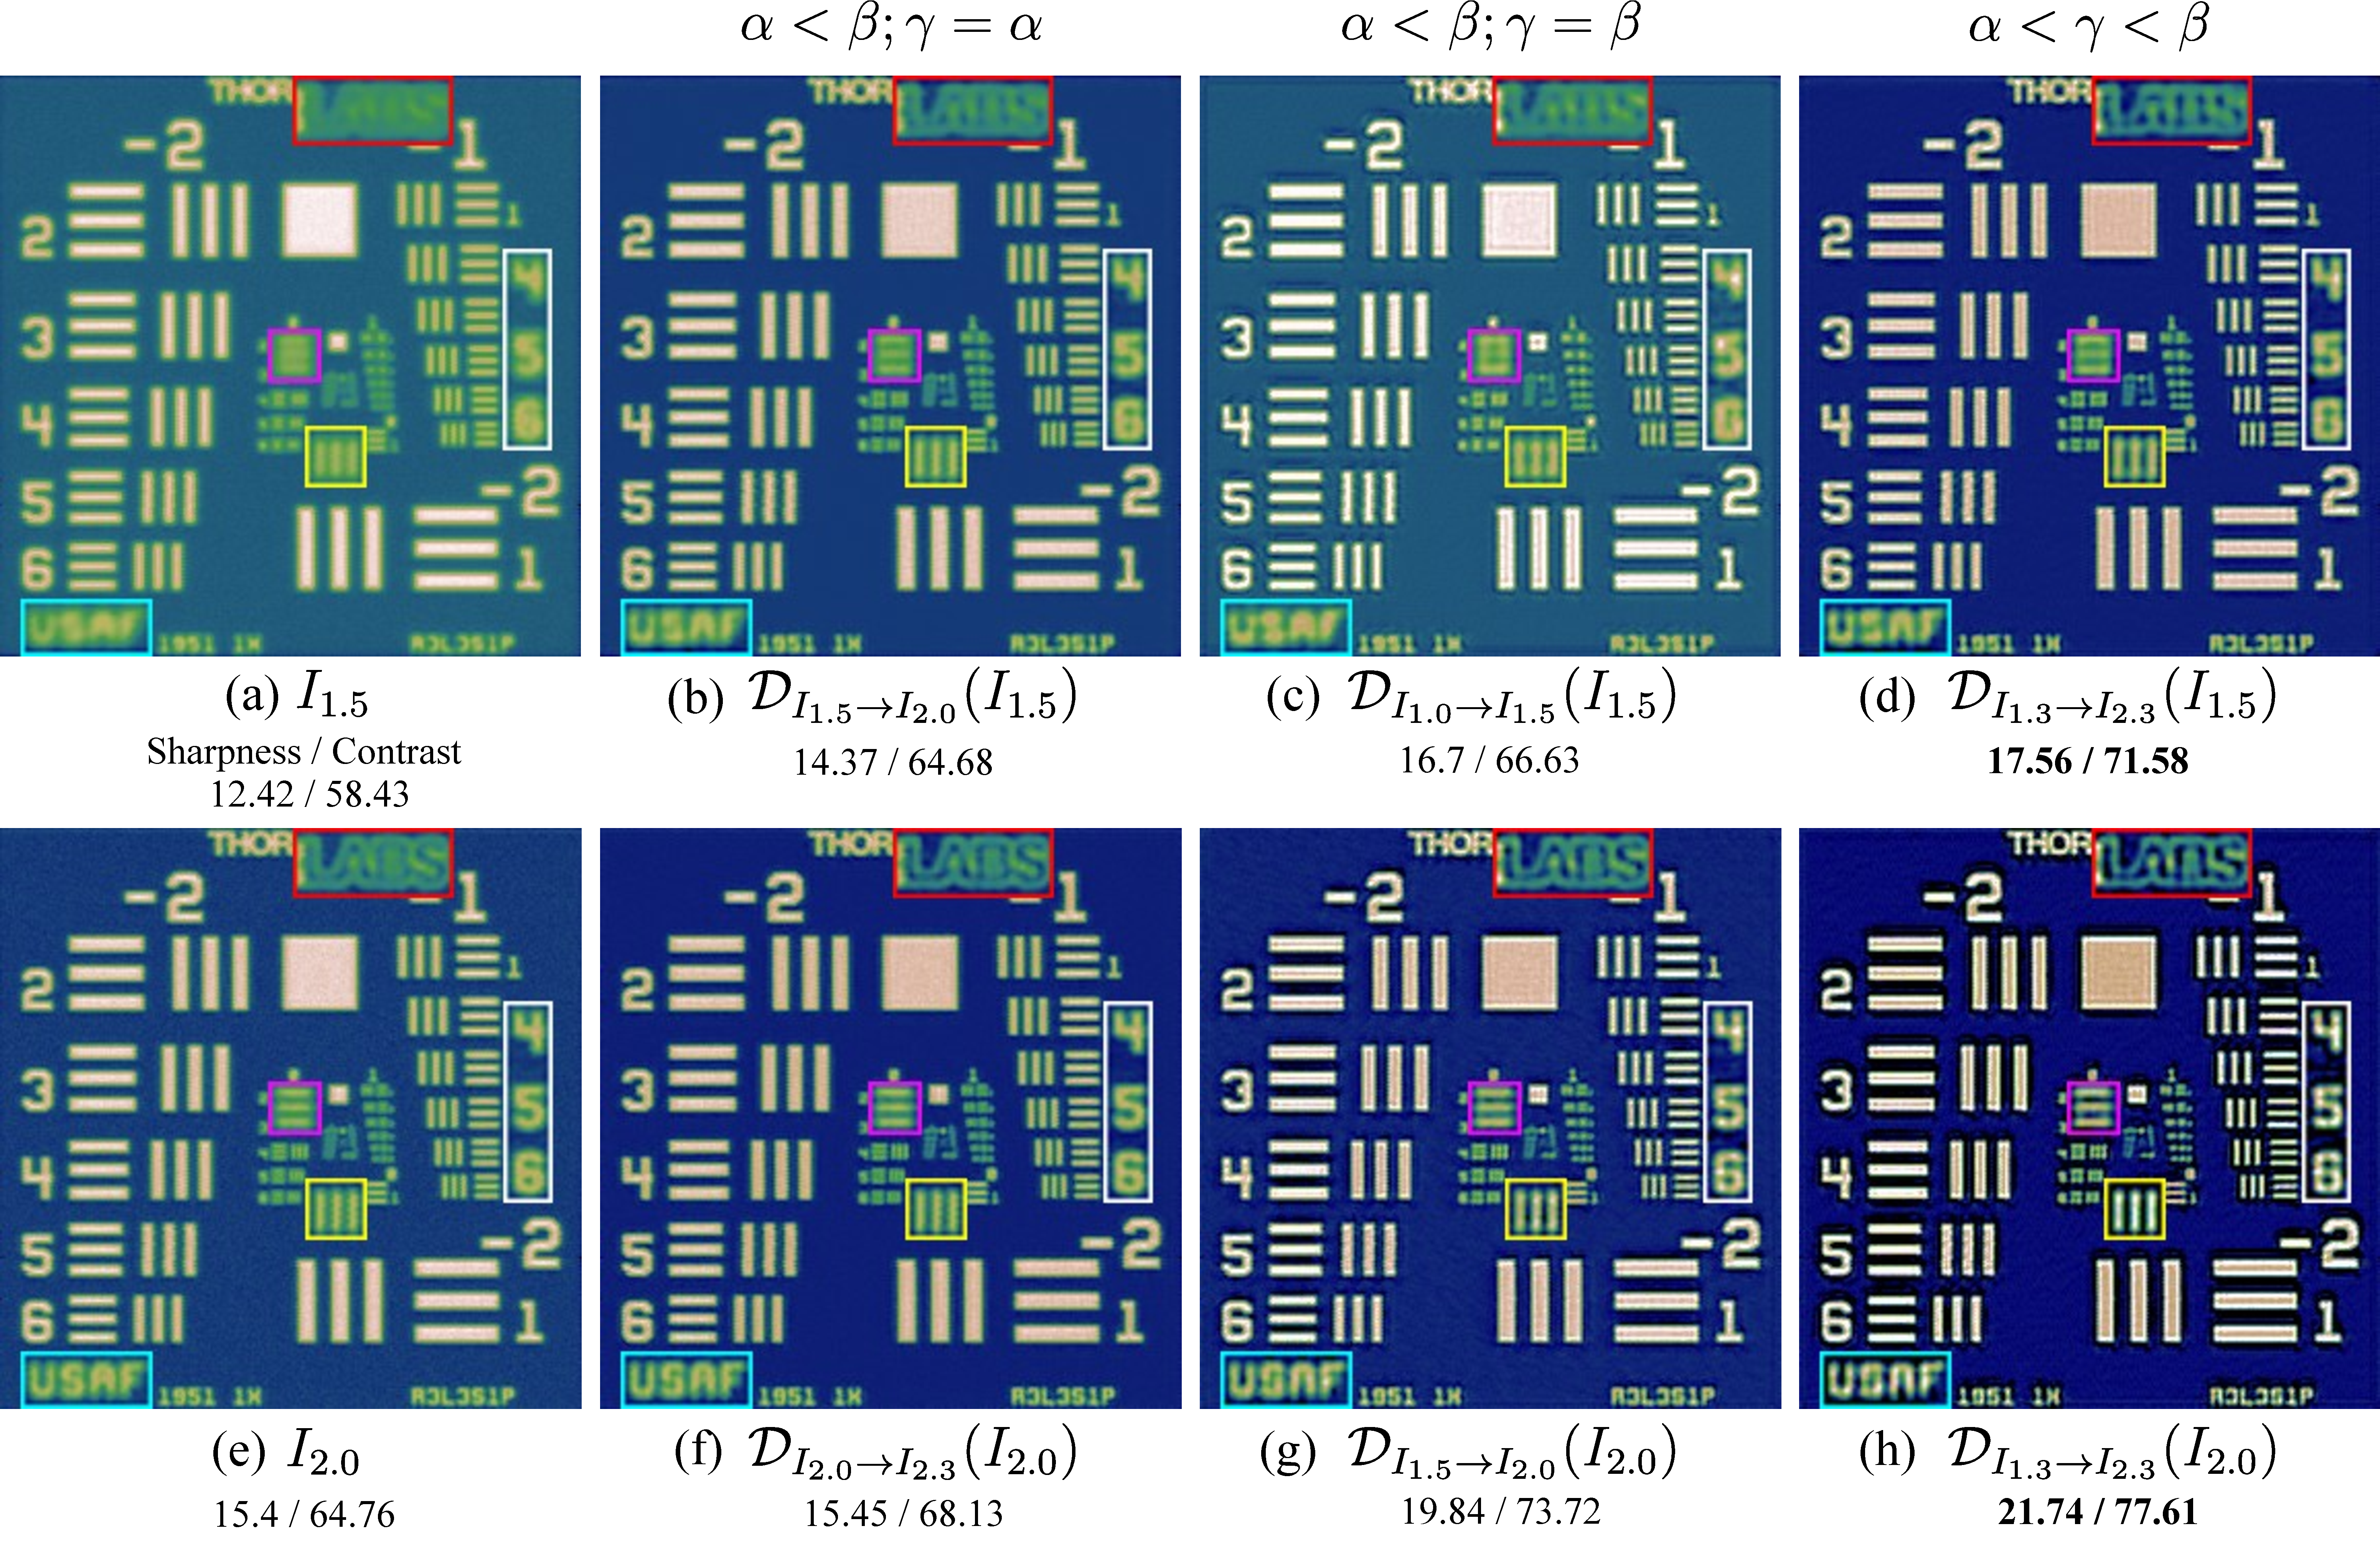
\includegraphics[width=\textwidth]{fig/Ryu-fig10.pdf}
    \caption{Self-supervised intra-data inference deblurring results based on 1.5 and 2.0 THz images. (a) Original 1.5 THz image; (b)-(d) O2O results of 1.5 THz image; (e) original 2.0 THz image; (f)-(h) O2O results of 2.0 THz image.}
    \label{fig:o2o_deblur}
\end{figure*}

The enhancement in image quality was demonstrated by applying the model trained using the O2O method, as depicted in Fig.~\ref{fig:o2o_explain}b, to the images used for training. It illustrates how low-frequency images emulate high-frequency images, thereby overcoming the diffraction limits of low-frequency images. During training, the frequencies of the input and target images are denoted as $\alpha$ and $\beta$, respectively; meanwhile, for inference, the frequency of the input image is denoted as $\gamma$. Generally, if $\alpha < \beta$ during network training, then blurriness can be eliminated by overcoming the low-frequency characteristics. Because high-frequency images exhibit higher sharpness than low-frequency images (see Fig.~\ref{fig:iqa}), learning this mapping can enhance the clarity of the image. However, high-frequency images above a certain frequency may exhibit higher noise levels; therefore, although the sharpness increases, additional noise may be introduced.

Fig.~\ref{fig:o2o_deblur} presents the visual results showing the overcoming of the diffraction limit of low-frequency images for 1.5 THz and 2.0 THz images. Figs.~\ref{fig:o2o_deblur} a and (e) are the original images before model inference, and Figs.~\ref{fig:o2o_deblur} (b) and (f) show the cases where $\gamma=\alpha$, which implies that the frequencies of the source and inference images are identical. Figs.~\ref{fig:o2o_deblur} (c) and (g) show the scenarios where $\gamma=\beta$, which implies that the inference and target image frequencies are the same. Finally, Figs.~\ref{fig:o2o_deblur} (d) and (h) show the results when the frequencies of the source, target, and inference images are different. The corresponding sharpness and contrast values are indicated below each image. As shown in Fig.~\ref{fig:o2o_deblur} a, the magnified area of the original 1.5 THz image exhibited blurry and smudged characteristics. The enhanced images (Figs.~\ref{fig:o2o_deblur} (b)-(d)) showed significantly clearer characteristics and more defined bar indices (see yellow box).  When the frequency of the inference image matched that of the source image, the image quality improved stably, as shown in Fig.~\ref{fig:o2o_deblur} (b). As shown in Fig.~\ref{fig:o2o_deblur} (c), when the frequency of the inference image matched that of the target, the clarity of the image clearly improved, however, it was accompanied by some distortion. Moreover, as shown in Fig.~\ref{fig:o2o_deblur} (d) and (h), when the inference image frequency of the source and target were different, the maximum sharpness and contrast was achieved at a specific frequency. This indicates the importance of selecting the appropriate frequency for the source and target images to enhance the quality of the inference image. The quantitative measures, such as sharpness and contrast, improved differently depending on the frequency matching in the inference results of the 1.5 THz image. When the frequency of the inference image matched that of the source image, the sharpness increased from 12.42 to 14.37, and the contrast increased from 58.43 to 64.68. When the frequency of the inference image matched that of the target, the sharpness and the contrast increased to 16.7 and 66.63, respectively. Finally, at a specific frequency different from those of both the source and target, the sharpness and contrast peaked at 17.56 and 71.58, respectively. Although some distortions occurred with the increased sharpness and contrast, the results were visually pleasant. In particular, Fig.~\ref{fig:o2o_deblur} (d) shows much less blurring compared with Fig.~\ref{fig:o2o_deblur} (a), which resulted in clearer and more defined characters. A similar trend was observed for the 2.0 THz image shown in Fig.~\ref{fig:o2o_deblur} (e).
The 2.0 THz image, owing to its frequency characteristics, was sharper and exhibited higher contrast than the 1.5 THz image. The trend identified in the inference results of the 1.5 THz image was correspondingly observed in the inference results of the 2.0 THz image.
At 2.0 THz, when the frequency of the inference image matched that of the source, the sharpness increased slightly from 15.4 to 15.45, and the contrast increased significantly from 64.76 to 68.13. Based on matching with the target image frequency, the sharpness and contrast increased substantially to 19.84 and 73.72, respectively. Notably, at a specific frequency different from those of both the source and target, the 2.0 THz image achieved the maximum sharpness and contrast values of 21.74 and 77.61, respectively. Matching the frequency of the inference image to that of the source resulted in stable and distortion-free image quality enhancement. However, performing inference at a frequency matching that of the target or one that is different from those of both the source and target can significantly improve image sharpness and contrast. These results emphasize the importance of selecting the appropriate frequency when generating inference images and show that, remarkably, when the frequency of the inference image matches that of the target image, or a specific frequency is chosen arbitrarily, significant improvements in image quality can be achieved. However, some degree of image distortion may occur.


\subsection{Self-Supervised Cross-Data Inference}
Next, we demonstrate that the proposed method can overcome the diffraction limit on images not used for training, as shown in Fig.~\ref{fig:o2o_explain}(c).
We inferred a new image $J$ (unrelated to the images used for training the model), which was trained with a positive USAF 1951 resolution target image. 
To ensure stable image-quality improvement, the frequency $\gamma$ of the inference image $J$ was set to be equal or similar to the frequency $\alpha$ of the input image used for training.
Fig.~\ref{fig:o2o_deblur_cross}(a) shows an optical image of the metal bookmark with a Korean Goryeo celadon shape, and Fig.~\ref{fig:o2o_deblur_cross}(b) presents a 1.0 THz image of the bookmark acquired using the same THz-TDS system. Figs.~\ref{fig:o2o_deblur_cross}(c)-(e) show the cross-data inference results from the trained model $\mathcal{D}$, which was trained on a USAF THz SAHS image. 
These results show a clear improvement in all the original THz images, both in terms of visual appearance as well as quantitatively in terms of sharpness and contrast values. Notably, inference using a model trained to map from 1.0 to 1.5 THz sharpened the image details and increased the contrast, thus resulting in a more distinct image. A model trained to map from 1.0 to 2.5 THz further accentuated these features, as the greater the frequency ratio between the source and target images, the more excessively it emulates the characteristics of the high-frequency image. As shown in Fig.~\ref{fig:o2o_deblur_cross}(e), selecting the appropriate frequencies for source and target images can enhance image quality. Like the intra-data inference, the cross-data inference allows one to improve image quality while adjusting the degree of image distortion by selecting appropriate $\alpha$ and $\beta$ values.

In this study, we validated that the application of a model trained using THz SAHS image data to new THz images can enhance visual quality, sharpness, and contrast. This model, which was trained to emulate the characteristics from low to high frequencies, demonstrated potential for wide application in various imaging systems. Additionally, the proposed method improves the quality beyond the diffraction limit of THz images, thus rendering it promising for applications in fields such as security inspection, medical imaging, and materials science.

\begin{figure*}[htbp]
    \centering
    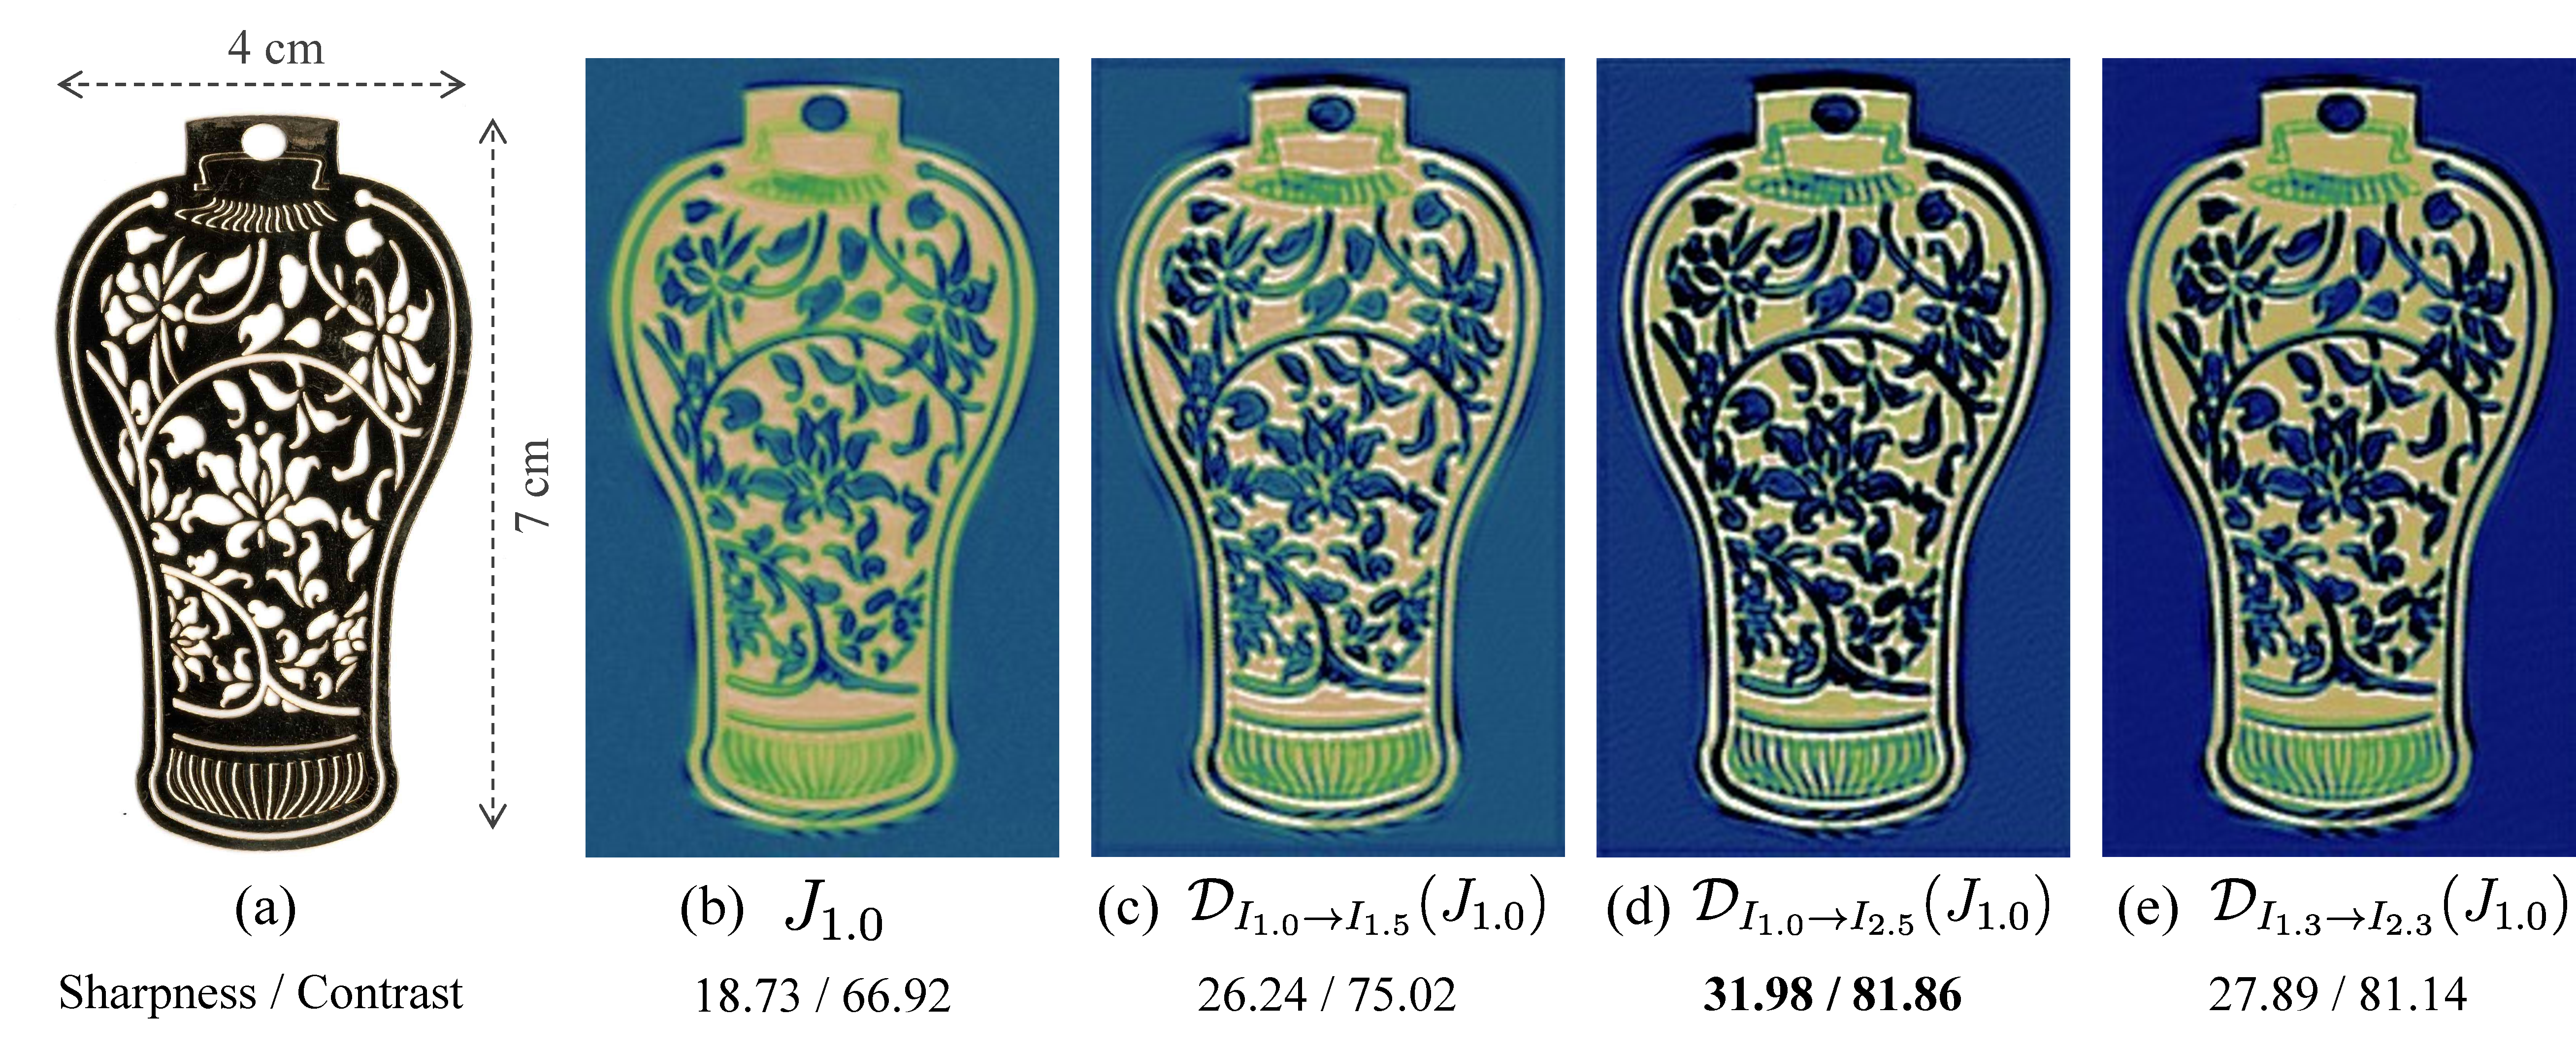
\includegraphics[width=\textwidth]{fig/Ryu-fig11.pdf}
    \caption{Self-supervised cross-data inference deblurring results based on O2O method. (a) Metal bookmark optical image; (b) measured THz image of metal bookmark at 1.0 THz; (c)-(e) cross-data inference results using pretrained model $\mathcal{D}$.}
    \label{fig:o2o_deblur_cross}
\end{figure*}

\subsection{High-Frequency Image Denoising}

\begin{figure*}[htbp]
    \centering
    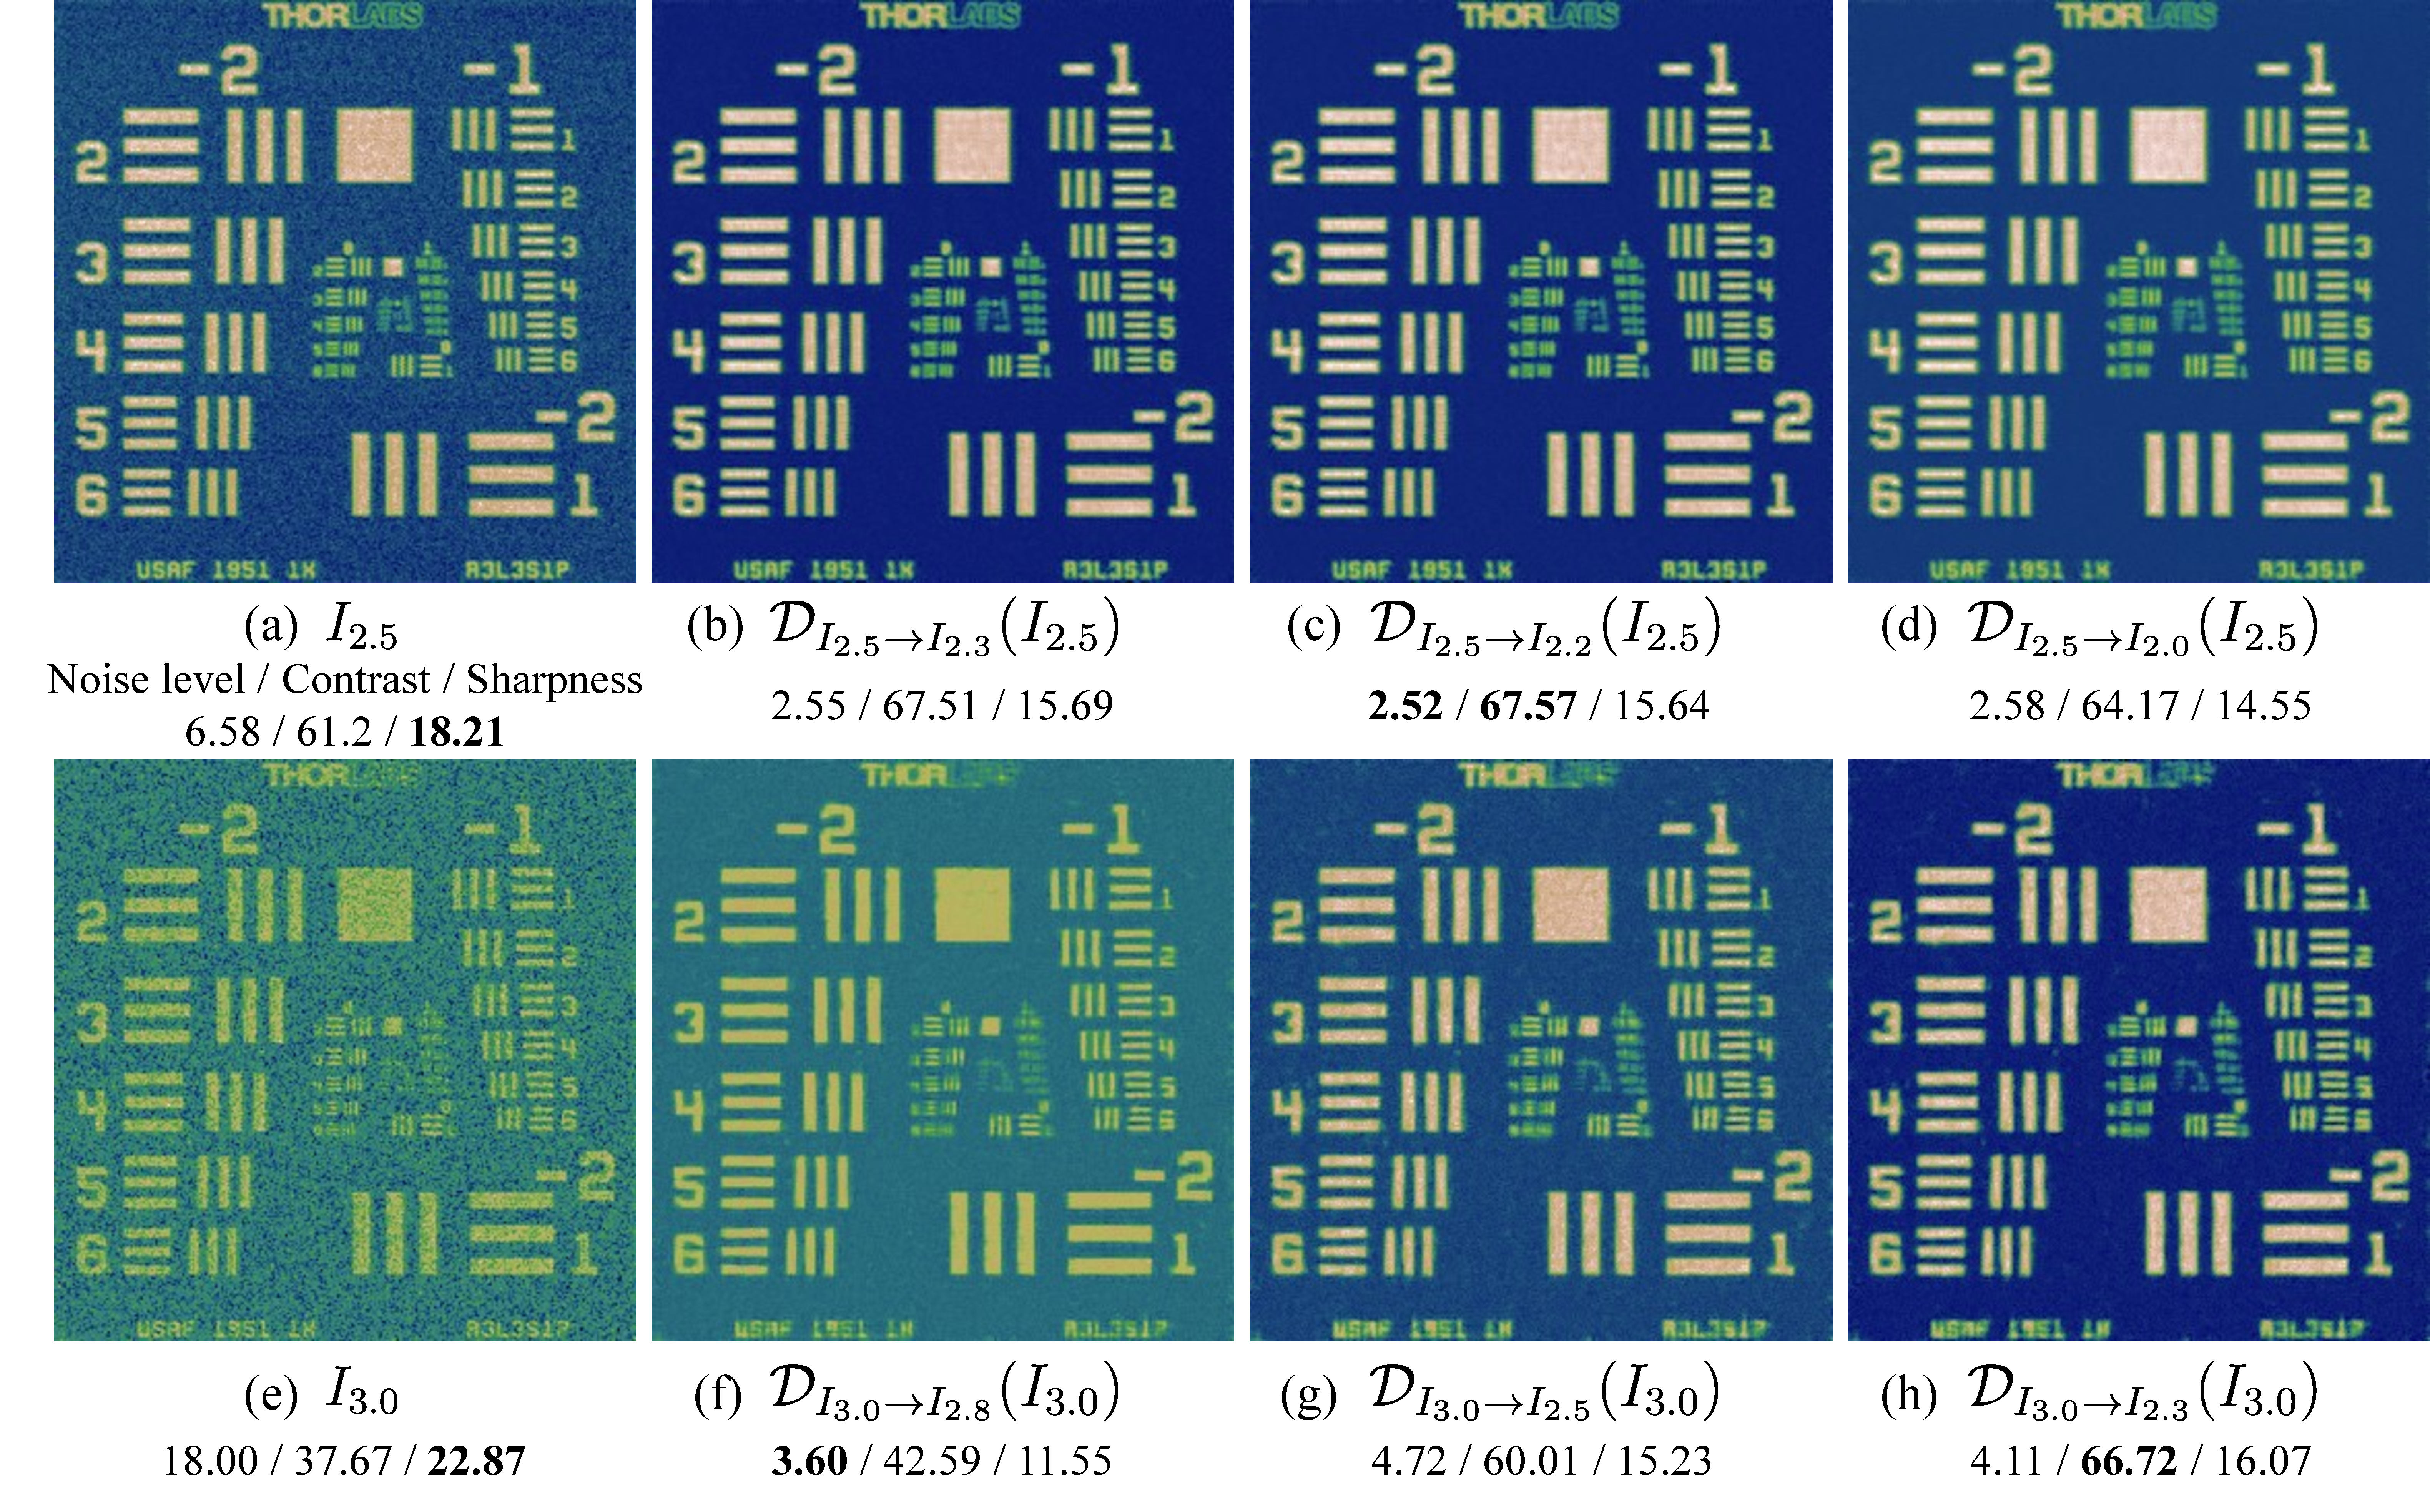
\includegraphics[width=\textwidth]{fig/Ryu-fig12.pdf}
    \caption{Self-supervised intra-data inference denoising results on 2.5 and 3.0 THz images based on O2O method. (a) Original 2.5 THz image; (b)-(d) O2O results of 2.5 THz image; (e) original 3.0 THz image; (f)-(h) O2O results of 3.0 THz image.}
    \label{fig:o2o_denoise}
\end{figure*}

In a THz-TDS system, as the frequency increases, the power of THz waves decreases, thus resulting in increased image noise levels. In this case, by emulating noise-free images at lower frequencies, effective noise reduction can be achieved in high-frequency images with slight loss in sharpness. This corresponds to the case involving the proposed O2O method with $\alpha > \beta$. This approach is key for improving image quality in the THz domain and can solve the issue of image noise at high frequencies.
Fig.~\ref{fig:o2o_denoise} shows the visual results of denoising high-frequency images at 2.5 and 3.0 THz. The first column shows the original images before model inference, and the remaining columns represent the results of noise reduction using models trained by fixing the source-image frequency $\alpha$ and adjusting the target-image frequency $\beta$. The noise levels and contrast values are indicated below each image. In all results, both the visual and quantitative noise levels decreased compared with the result of original images. The contrast improved as the noise decreased. The degree of noise reduction and contrast enhancement varied depending on the $\beta$ value. In the 2.5 THz image, the noise level decreased by approximately 62\% compared with the original, whereas in the 3.0 THz image, it decreased by 74\%-80\% as shown in Figs.~\ref{fig:o2o_denoise}b-\ref{fig:o2o_denoise}d and \ref{fig:o2o_denoise}f-\ref{fig:o2o_denoise}h. However, since the images were trained to target lower frequency images, the sharpness decreased by 14\%-20\% and 30\%-49\% for the 2.5 and 3.0 THz images, respectively, after noise reduction. These results imply that to reduce noise in high-frequency images, which are sharp but noisy, some loss of sharpness should be tolerated.

Cross-data inference has also been applied to the denoising methods using THz SAHS images. Fig.~\ref{fig:o2o_denoise_cross} shows the results of applying cross-data inference to reduce noise in high-frequency images of the metal bookmark with the Korean Goryeo celadon shape. In all the inference results, the noise level decreased by 18\%-24\% and the contrast improved. In particular, more excellent noise reduction effects were observed at larger frequency spans. These results indicate that noise can be effectively reduced in the new THz images with entirely different shapes from the images used in training, thus proving that the proposed method can be universally applied to various types of images. This THz SAHS image-based denoising method decreases in sharpness only slightly owing to the use of low-frequency images. However, considering the high spatial resolution provided by high-frequency images, this learning method, which effectively removes image noise with a slight reduction in spatial resolution to achieve cleaner images can be useful in various fields. In fact, it is expected to be applicable to various imaging areas beyond THz imaging.

\begin{figure*}[htbp]
    \centering
    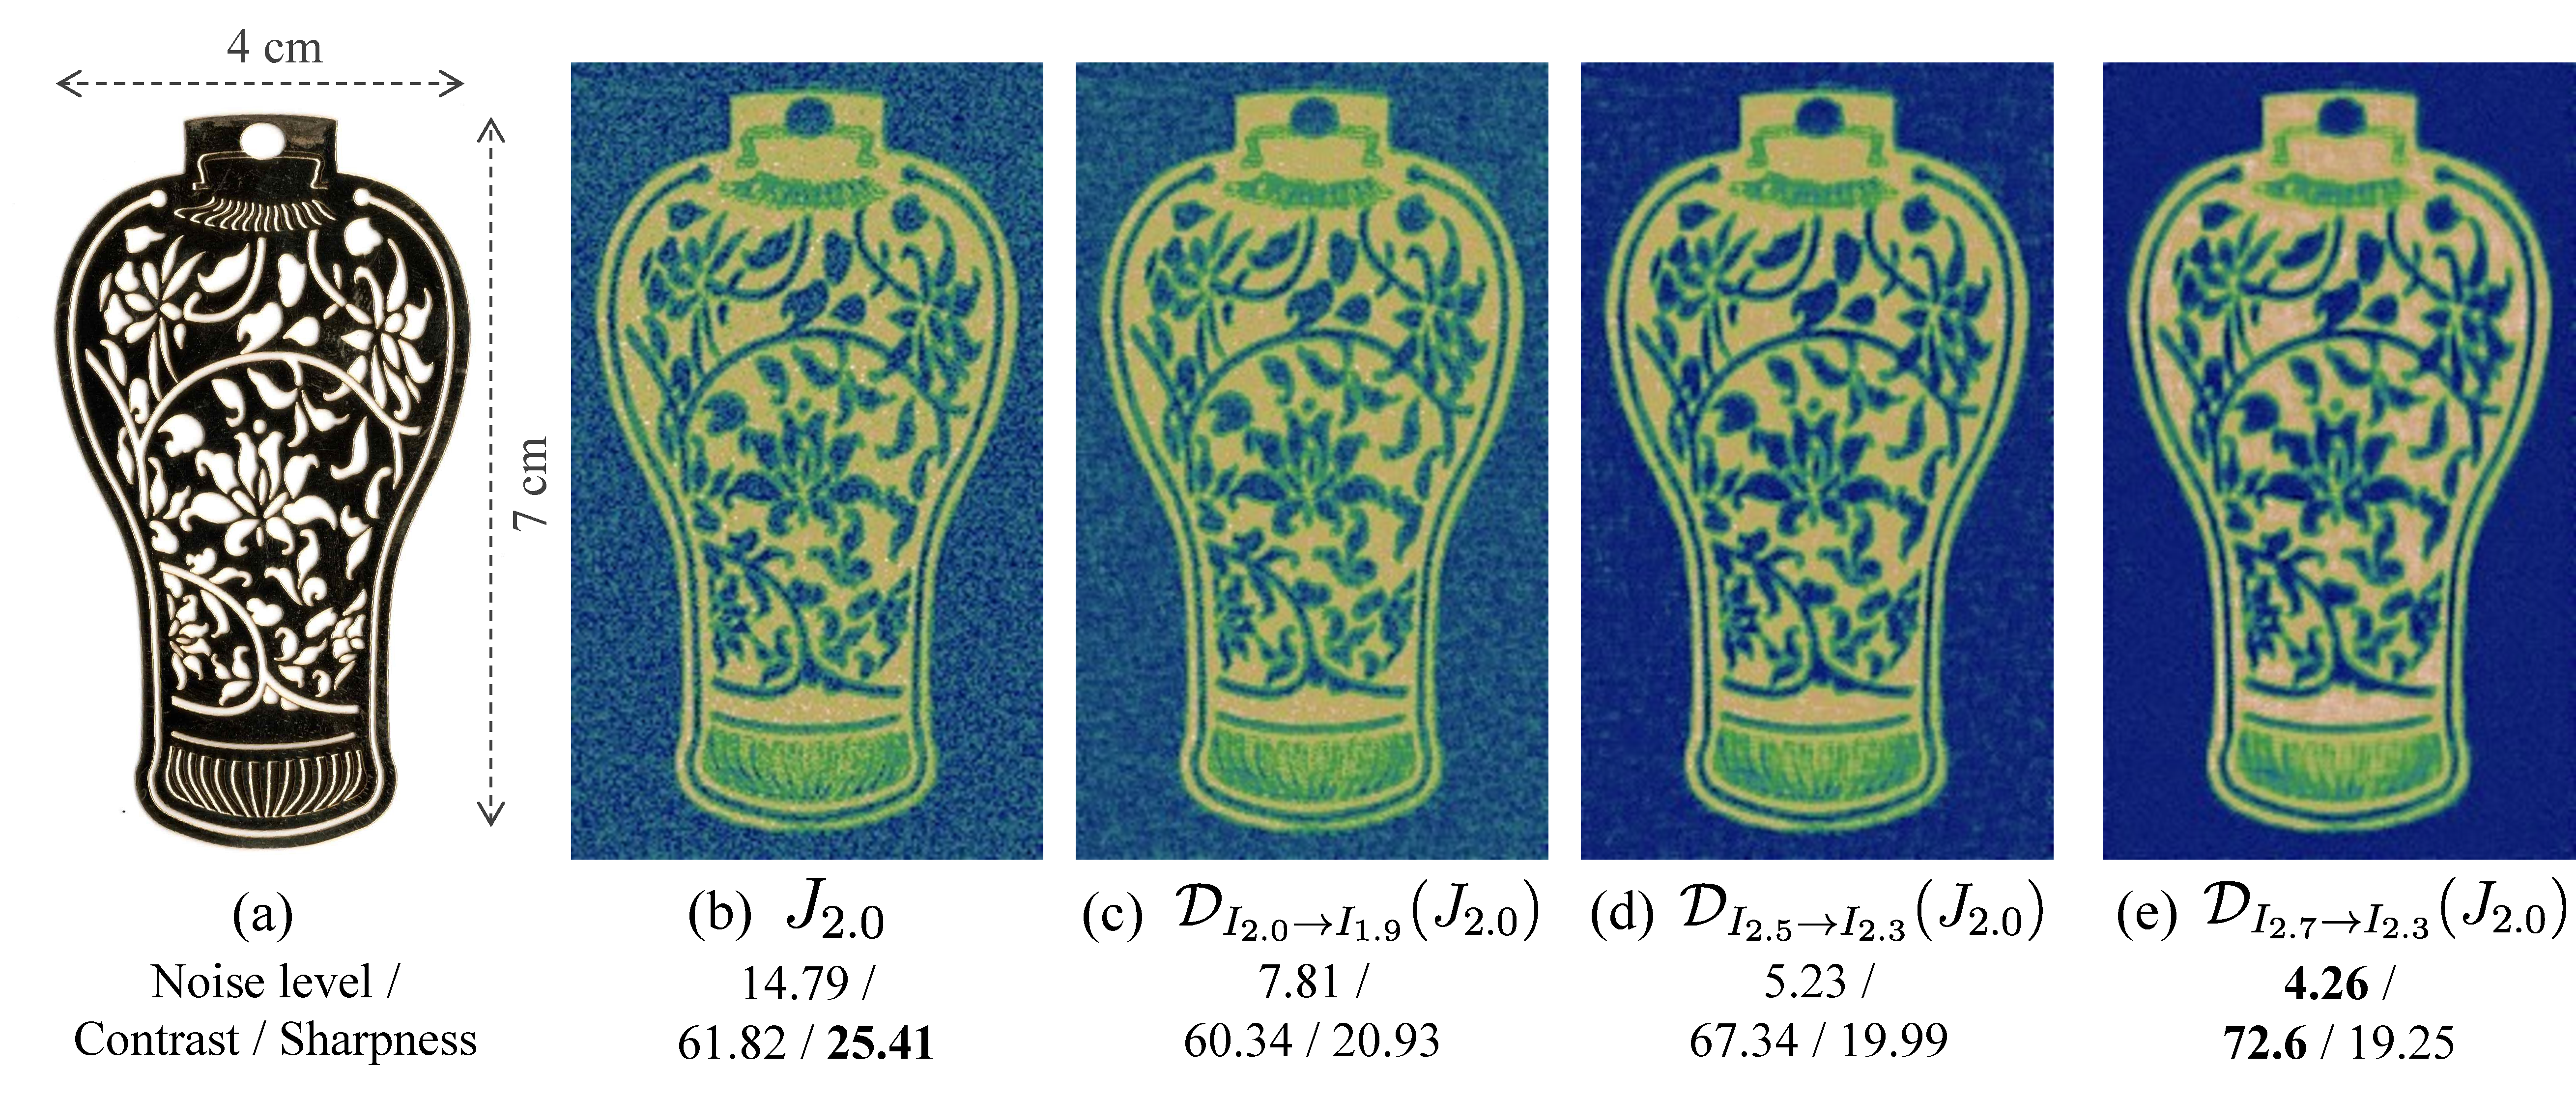
\includegraphics[width=\textwidth]{fig/Ryu-fig13.pdf}
    \caption{Self-supervised cross-data inference denoising results based on O2O method. (a) Metal bookmark optical image; (b) measured THz image of metal bookmark at 2.0 THz; (c)-(e) cross-data inference results using pretrained model $\mathcal{D}$.}
    \label{fig:o2o_denoise_cross}
\end{figure*}

\subsection{RE Results}
The effectiveness of the proposed RE method (Fig.~\ref{fig:recurrent_explain}) for further improving the O2O results described in Section~\ref{sec:intra} was evaluated. Fig.~\ref{fig:recurrent} shows the results of applying the RE method to 1.8 and 2.0 THz images. Figs.~\ref{fig:recurrent}b and f show the results of the O2O inference. And Figs.~\ref{fig:recurrent}c and g show the results of one recurrence, obtained from re-inferring the image using a model trained with the target as the source and the once-inferred result as the target in Figs.~\ref{fig:recurrent}b and f. Figs.~\ref{fig:recurrent}d and h show the results of the two recurrences. In the case of the 1.8 THz image, the sharpness and contrast increased with each recurrence, showing visually sharper and improved results. However, for the 2.0 THz image, the sharpness and contrast were at their best in the result of the first recurrence. Moreover, as the number of recurrences increased, the distinction between the index bars became clearer; however, the pixel values reduced significantly.
\begin{figure*}[htbp]
    \centering
    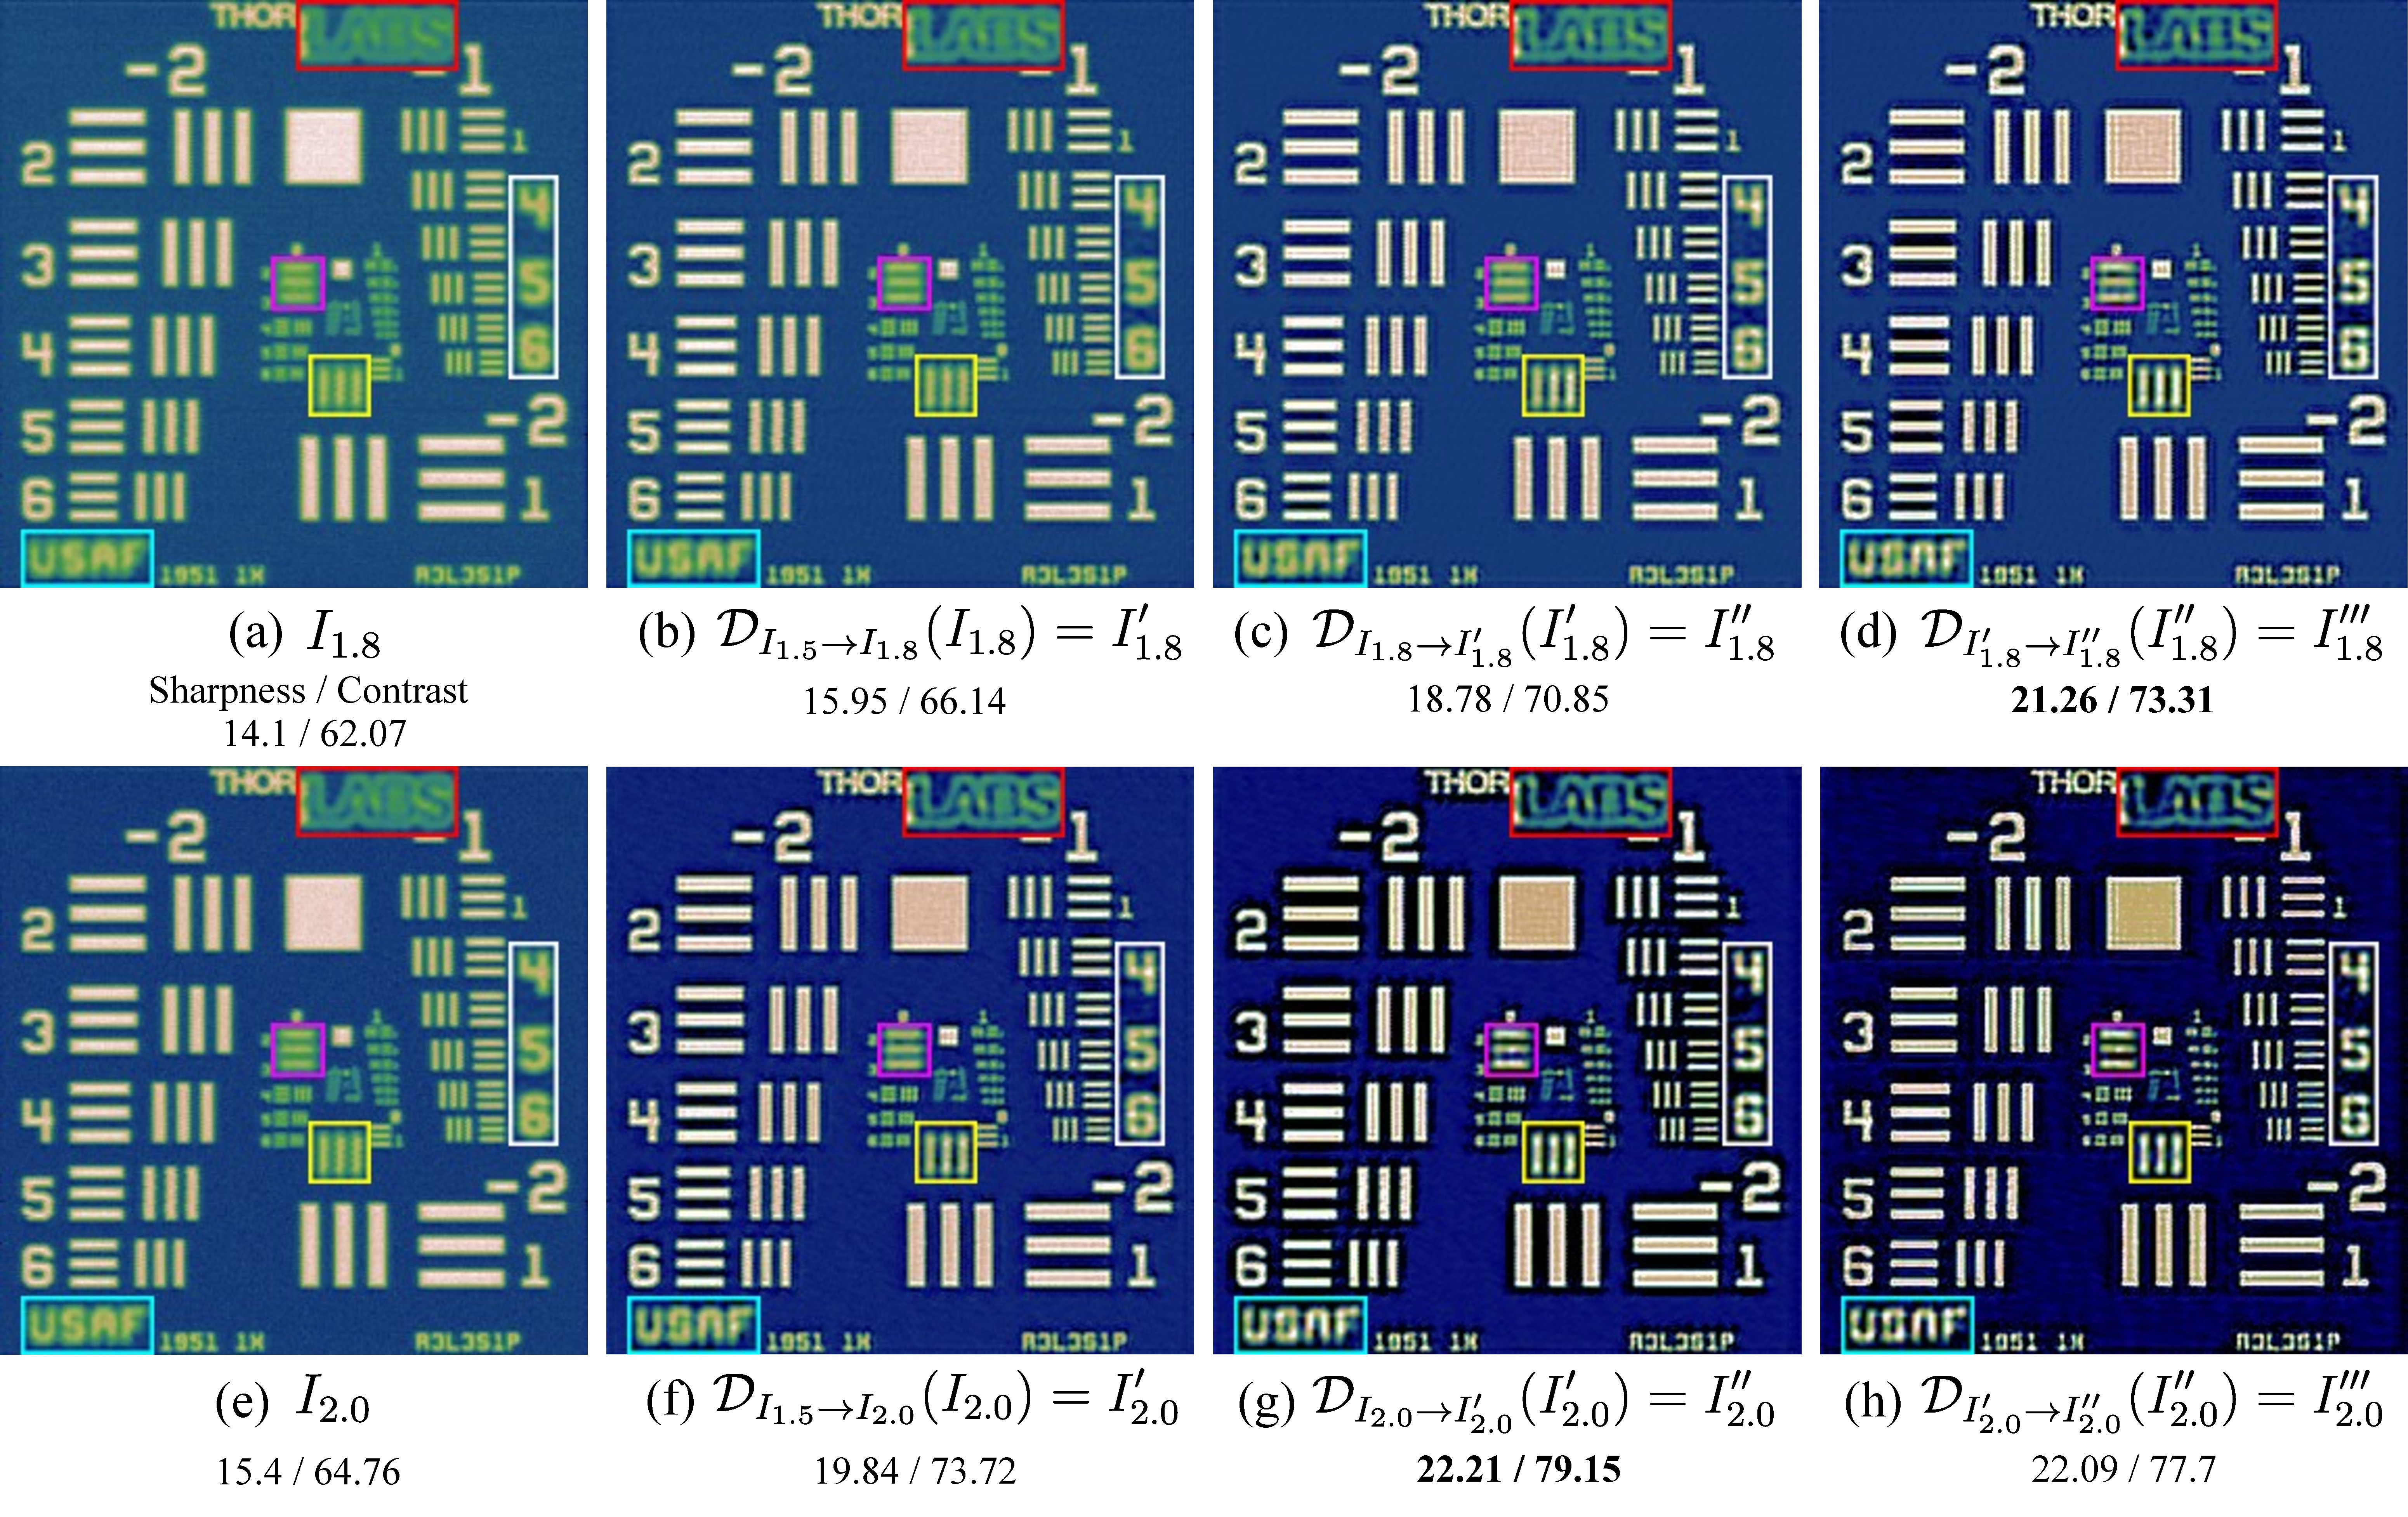
\includegraphics[width=\textwidth]{fig/Ryu-fig14.pdf}
    \caption{RE deblurring results based on 1.8 and 2.0 THz images.}
    \label{fig:recurrent}
\end{figure*}
To analyze the spatial resolution characteristics of the RE inference images shown in Fig.~\ref{fig:recurrent}, spatial-frequency spectrum analysis was conducted and the results are displayed in Fig.~\ref{fig:recurrent_spectrum}.
As the RE inference step advanced, the contrast of the boundaries intensified progressively, and the sharpness improved compared with that of the original image. The increase in contrast at key feature points, such as the central intersection, was more pronounced compared with that at the surrounding areas, thus reflecting sharper edges and a distinct contrast. This indicates that the RE inference process effectively amplifies the high-frequency components of the image, thereby effectively restoring the resolution and sharpness. Additionally, the ratio of the high-frequency energy was calculated and is indicated below each image. This ratio, which represents the energy in the high-frequency region of the spatial-frequency spectrum image, excludes the central section, which represents the low-frequency components. Higher values indicate sharper images. The proportion of high-frequency components increased with the number of recurrences, thus quantitatively confirming that the images became sharper.

\begin{figure*}[htbp]
    \centering
    \includegraphics[width=0.95\textwidth]{fig/Ryu-fig15.pdf}
    \caption{Spatial frequency spectrum of RE deblurring results based on 1.8 and 2.0 THz images.}
    \label{fig:recurrent_spectrum}
\end{figure*}

To analyze the excessive reduction in pixel values between the index bars of the inference image as the RE counts increased, we compared the pixel values of the optical image of the index bars of the positive USAF 1951 resolution target with the pixel values of the results of THz image inference using RE learning (see Figs.~\ref{fig:axial} and~\ref{fig:axial2}).
Figs.~\ref{fig:axial}a and~\ref{fig:axial2}a show the optical images of the USAF target. The pixel values along the red lines in these images were analyzed to evaluate the performance of the models inferred through RE learning. In Figs.~\ref{fig:axial}b and c and Figs.~\ref{fig:axial2}b and c, the cross-sectional pixel values of the optical images are presented alongside the RE inference results of the 1.8 and 2.0 THz images for comparison. The dashed black line represents the optical image, the dotted red line represents the original THz image, and the green line represents the image inferred by the O2O learning model. Additionally, the blue and purple lines represent the results of inferences made after applying RE once and twice, respectively.

Images inferred using the THz SAHS image-based model showed clearer distinctions between lines compared with the original THz images. This was particularly evident when RE model was used, which rendered the distinction between the lines as close as possible to the optical image. However, as the application of the RE model increases, although the distinction between lines becomes clearer, a dip appears at the center of the lines, thus resulting in image distortion. Therefore, the number of applications of the RE method in THz image processing should be determined meticulously based on the purpose of image acquisition.

Table~\ref{tab:beam_width} lists the beam widths calculated from Fig.~\ref{fig:axial2}(a) as full width at half maximum (FWHM) values. As shown, the beam width decreased as the operating frequency and the number of repetitions of the RE model increased. The beam widths for the 1.8 and 2.0 THz images were 0.776 mm and 0.721 mm, respectively. The beam width of the 1.8 THz image was reduced to 0.651 mm after one inference, which is a lower value than the beam width of the 2.0 THz image. The results quantitatively prove that the RE method can surpass the diffraction limit of THz images.

\begin{figure*}[htbp]
    \centering
    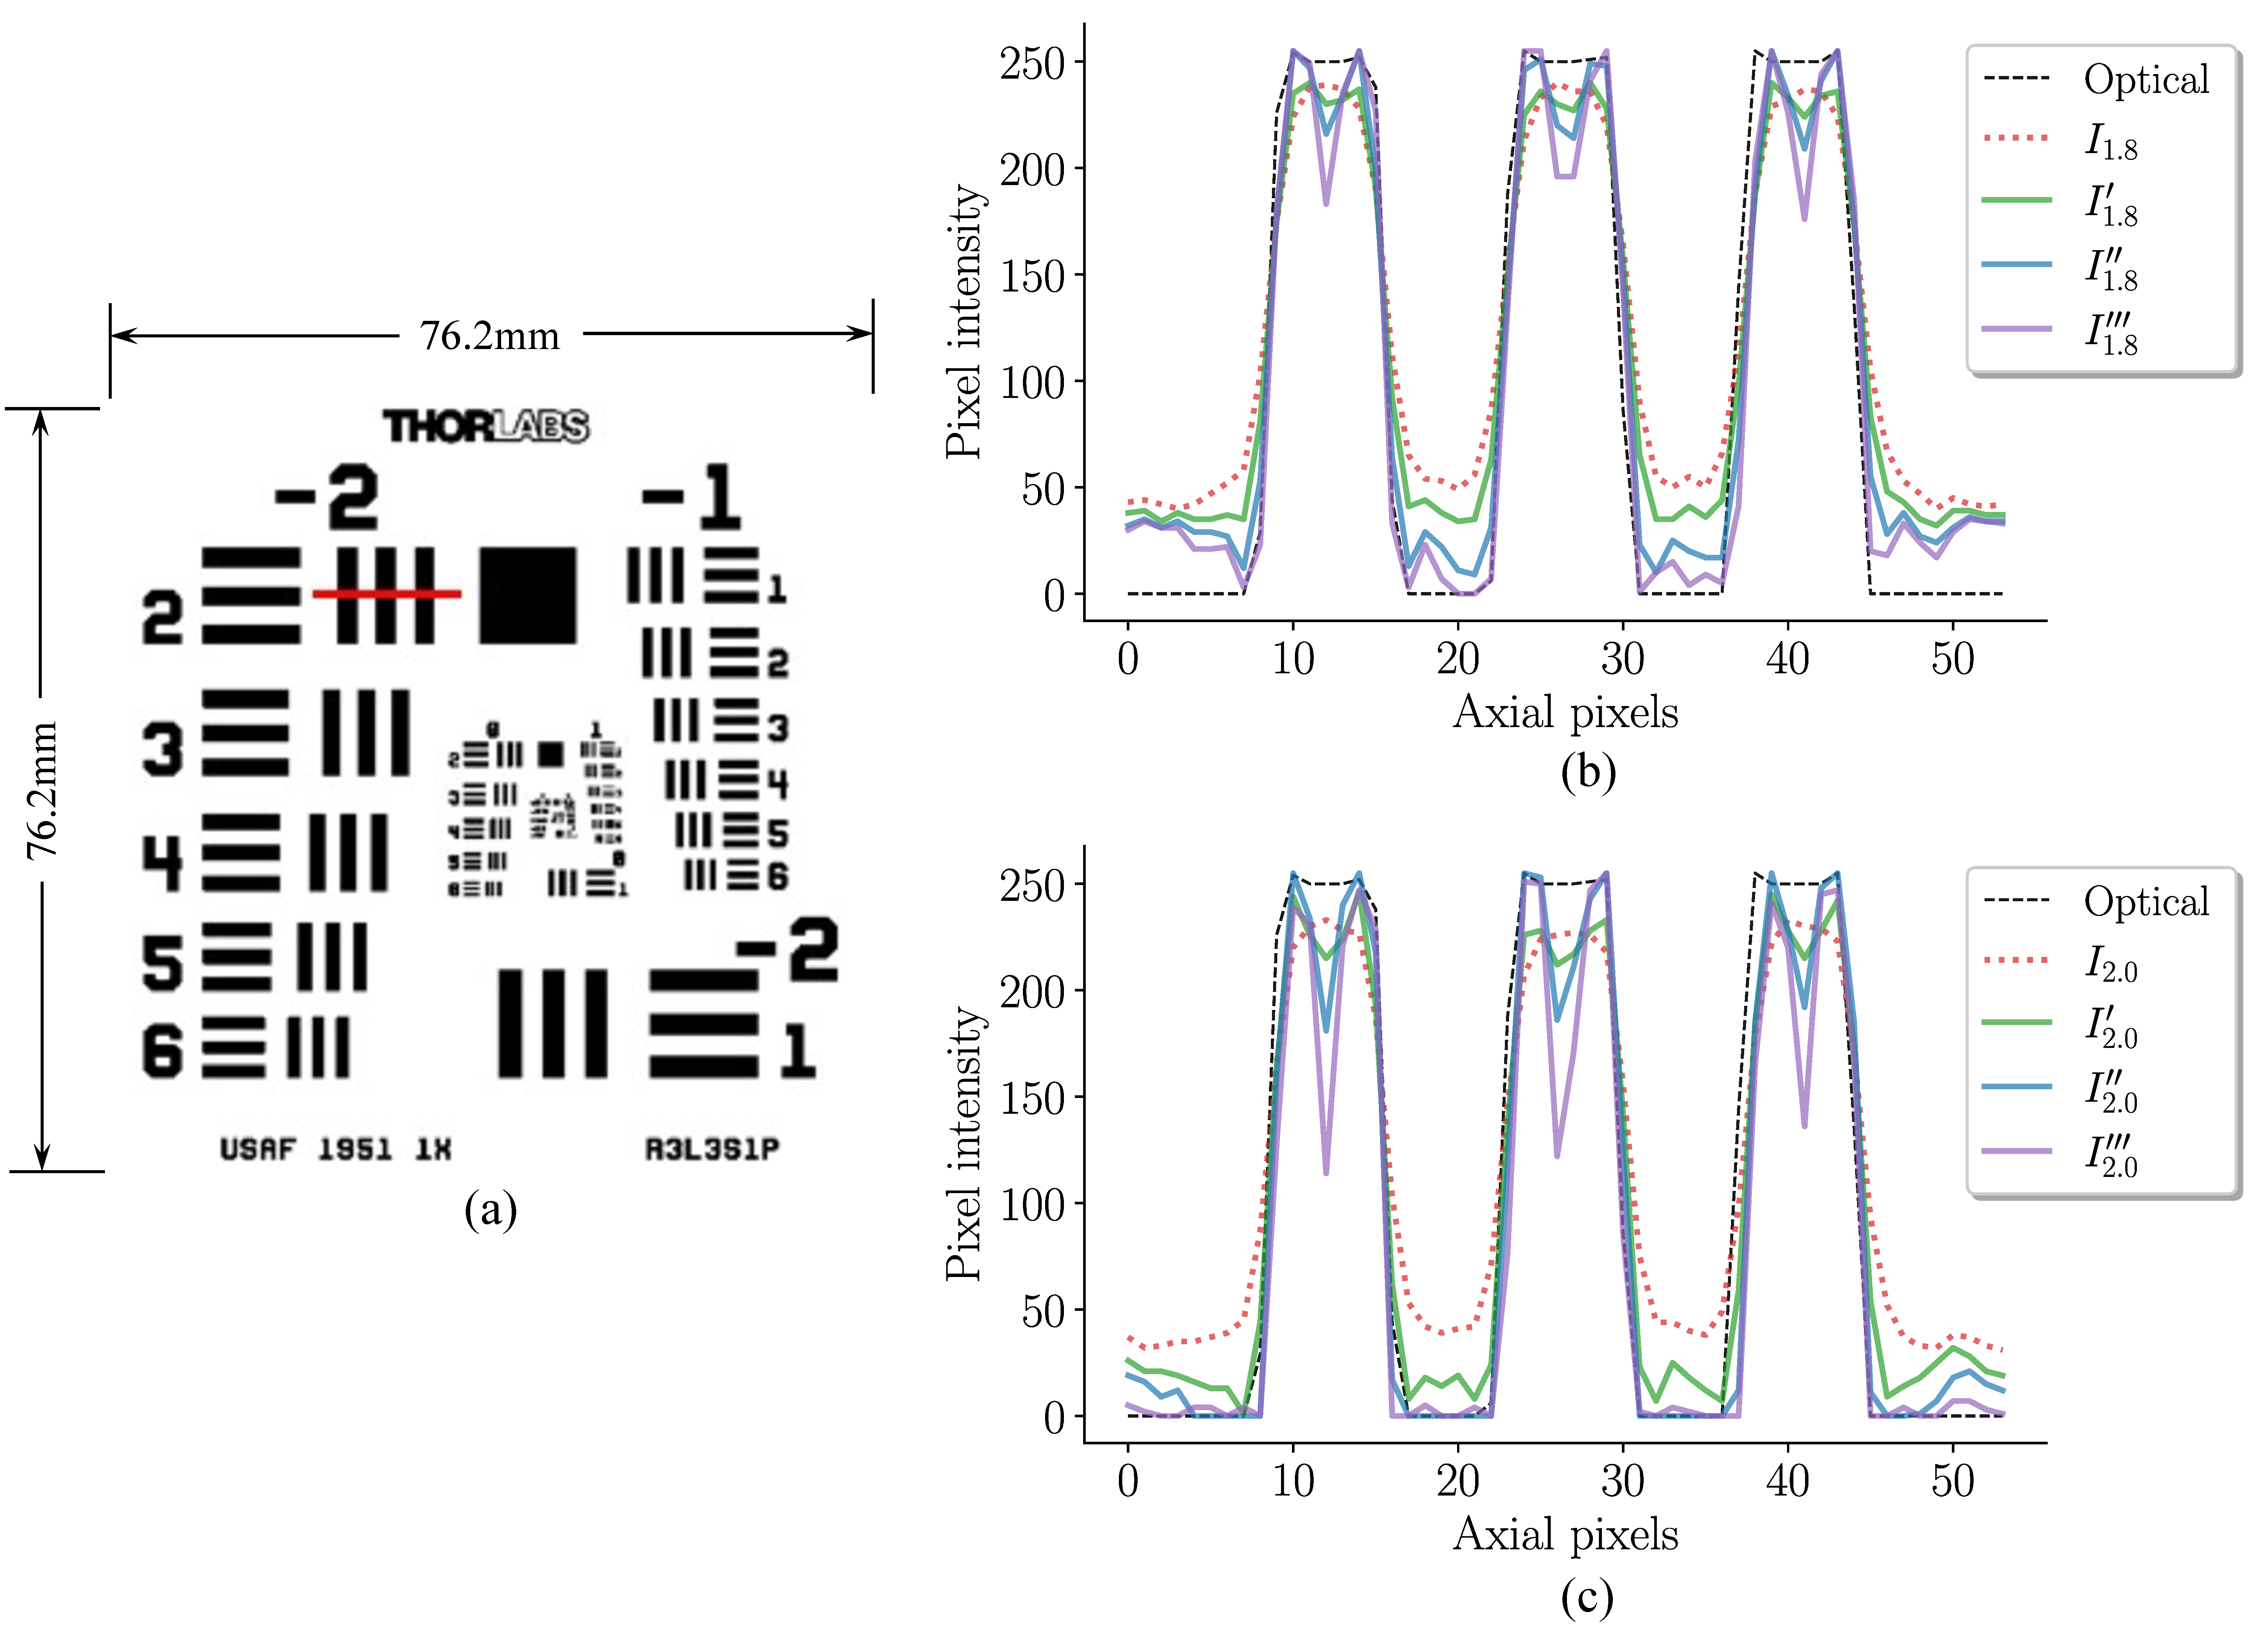
\includegraphics[width=0.7\textwidth]{fig/Ryu-fig16.pdf}
    \caption{Axial line graph comparison of improved results for 1.8 and 2.0 THz images.}
    \label{fig:axial}
\end{figure*}

\begin{figure*}[htbp]
    \centering
    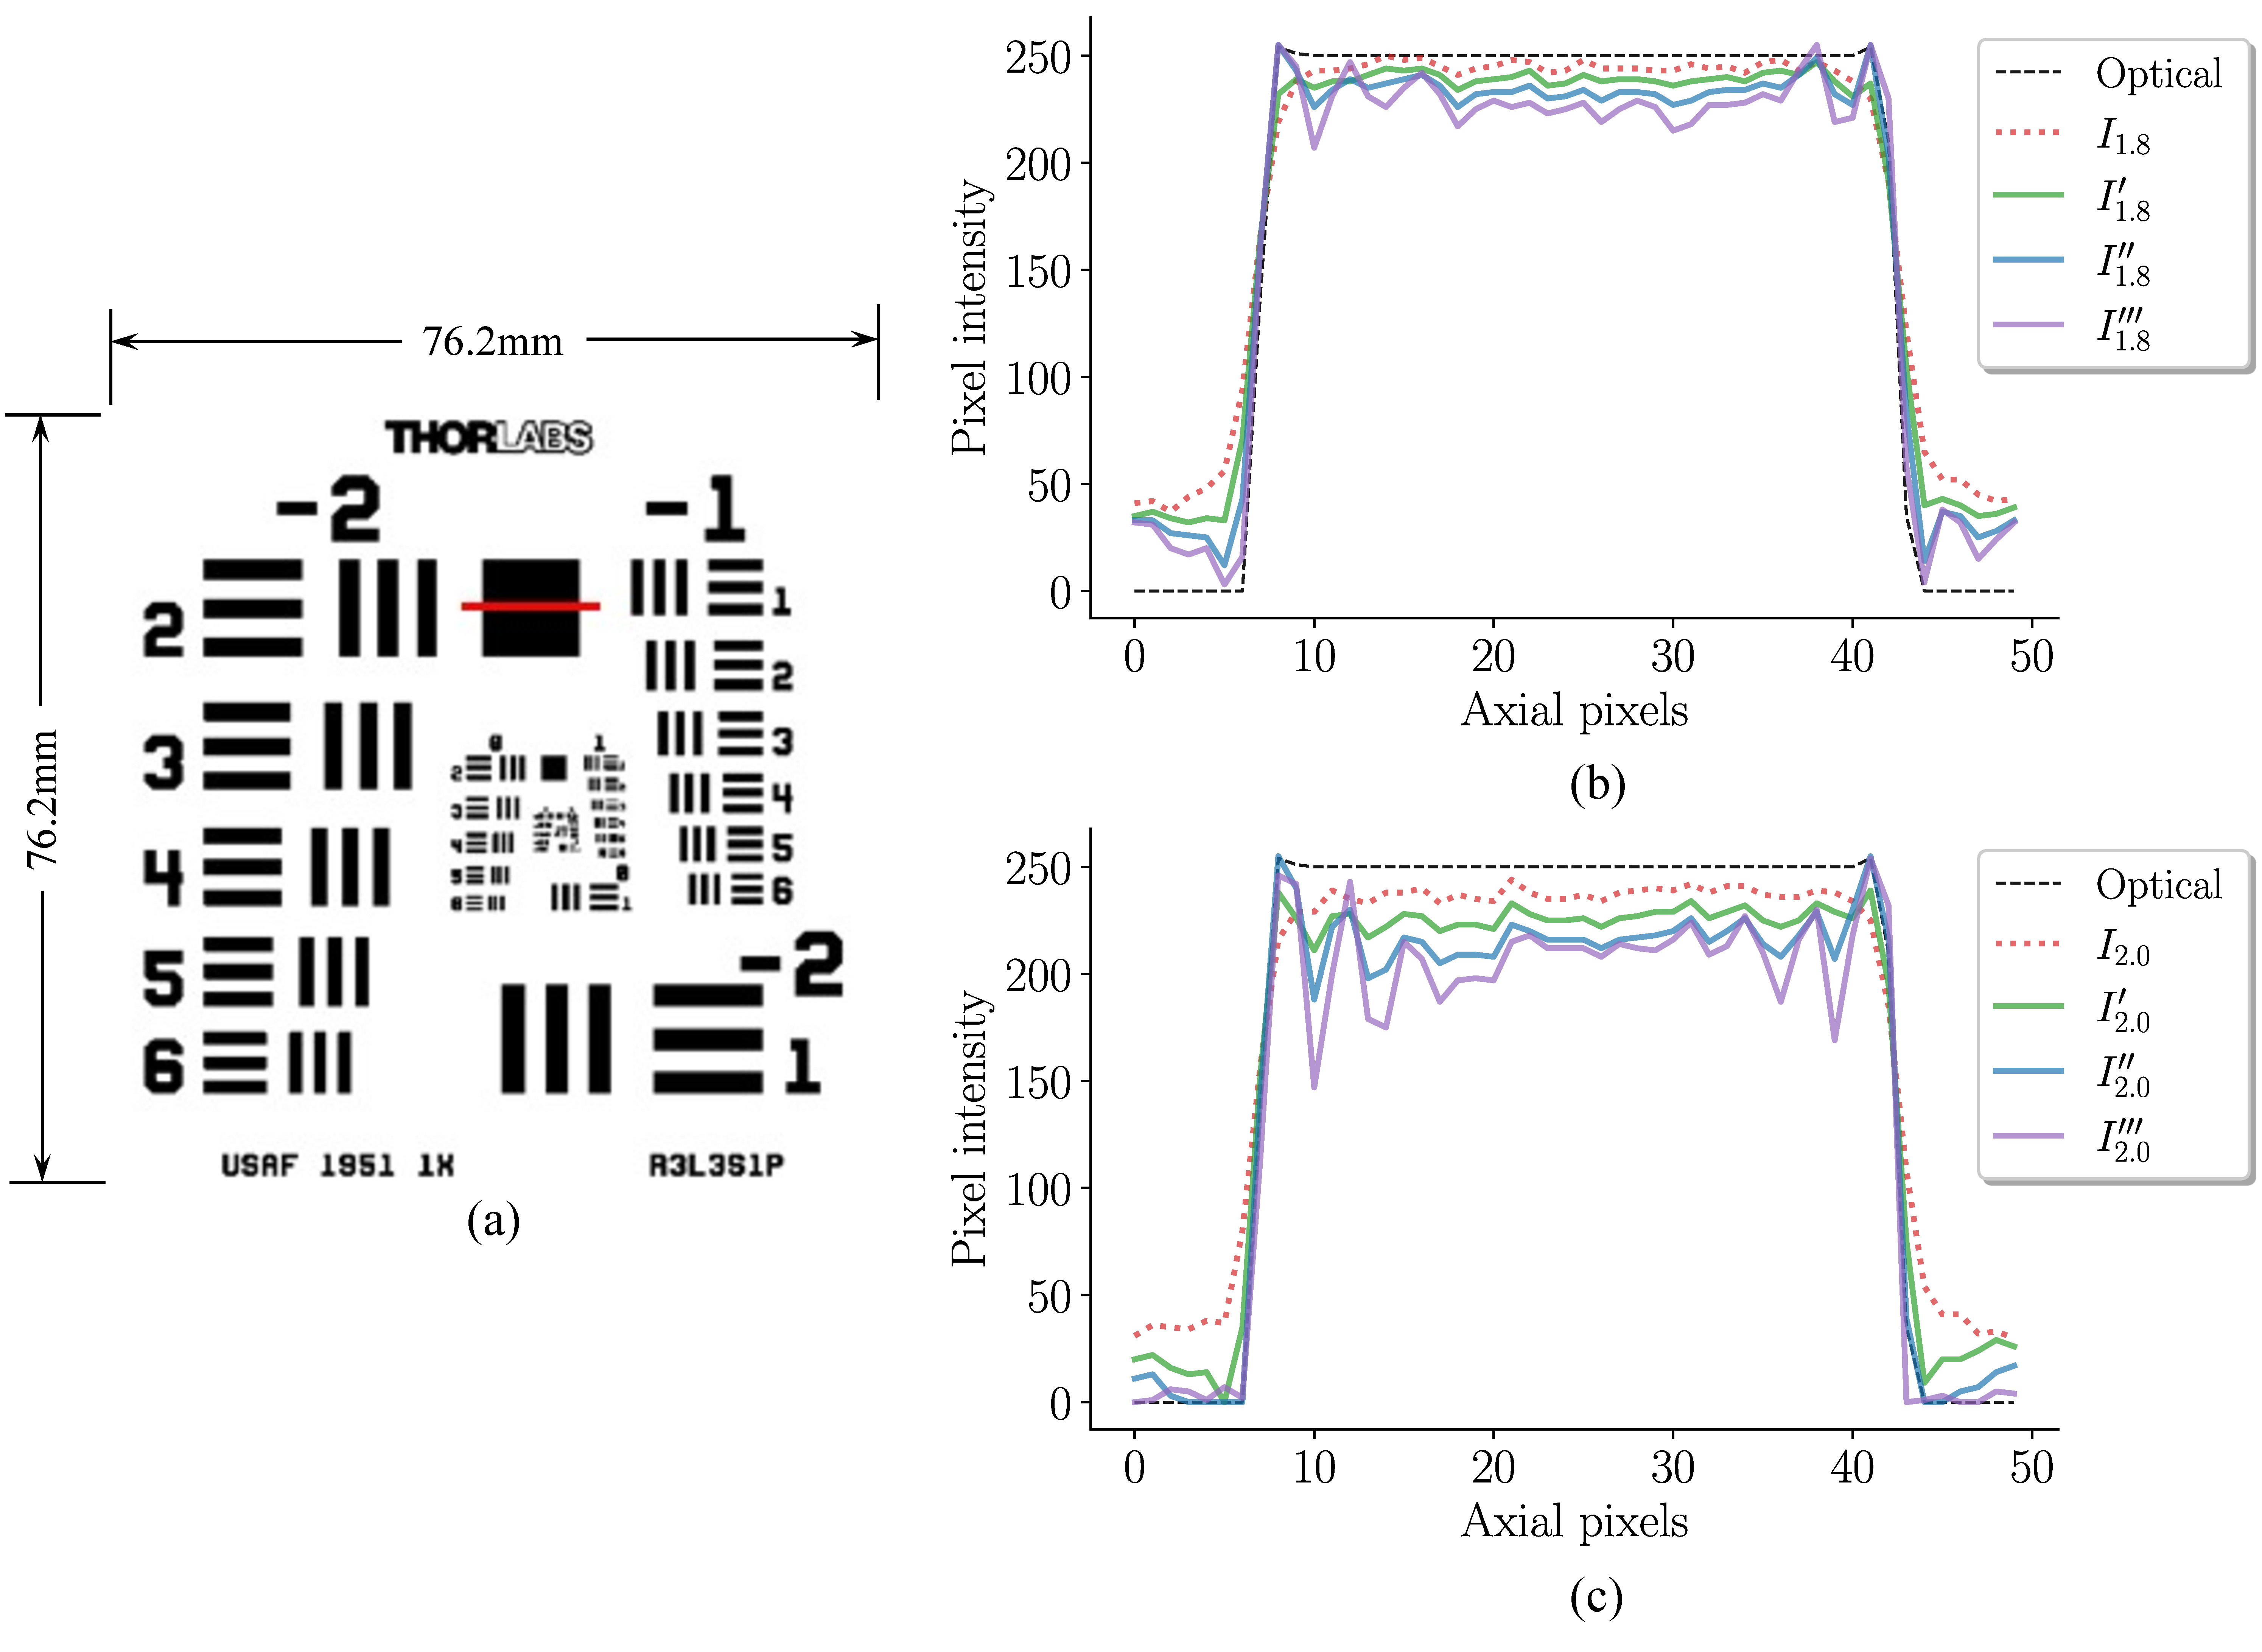
\includegraphics[width=0.7\textwidth]{fig/Ryu-fig17.pdf}
    \caption{Axial line graph comparison of improved results for 1.8 and 2.0 THz images.}
    \label{fig:axial2}
\end{figure*}


\begin{table}
    \centering
    \renewcommand{\arraystretch}{1.5} % Adjust the row height
    \begin{tabular}{c|c||c|c}
         \toprule
         \textbf{Image} & \textbf{Beam Width (mm)} & \textbf{Image} & \textbf{Beam Width (mm)} \\
         \midrule
         $I_{1.8}$ & 0.776 &$I_{2.0}$ & 0.721 \\
         $I_{1.8}'$ & 0.651 &$I_{2.0}'$ & 0.573 \\
         $I_{1.8}''$ & 0.566 &$I_{2.0}''$ & \textbf{0.506} \\
         $I_{1.8}'''$ & \textbf{0.530} &$I_{2.0}'''$ & \textbf{0.506} \\
         \bottomrule
    \end{tabular}
    \caption{Beam width measured as full width at half maximum (FWHM) of RE results.}
    \label{tab:beam_width}
\end{table}

\subsection{Image Super-Resolution}
Owing to the inherently low resolution of THz images, ZSSR was applied to enhance the resolution, as shown in Fig.~\ref{fig:zssr}. Fig.~\ref{fig:zssr}a displays the original 2.0 THz image, Fig.~\ref{fig:zssr}b shows the image with improved quality without scale change, and Fig.~\ref{fig:zssr}c presents the result with a scale factor of two, which resulted in a $584\times 584$ resolution image. The environment for training and inferring ZSSR is identical to that for the O2O learning. Even under the same O2O training, applying ZSSR with a scale factor of two resulted in a sharper image.
Fig.~\ref{fig:zssr_spectrum} illustrates the spatial frequency spectrum and high-frequency energy ratio for the images shown in Fig.~\ref{fig:zssr}. As the process progresses from the original image to the O2O inferred image and the 2x-expanded ZSSR inferred image, the textures and edges became clearer and high-frequency components became more conspicuous. The enlargement of the image scale further highlighted these features. In particular, the high-frequency energy ratio in the original 2.0 THz image increased from 0.1039 to 0.2114 after applying ZSSR, thus providing quantitative evidence of resolution improvement. These results prove that applying ZSSR to SAHS images acquired using a THz-TDS system can significantly improves the image quality compared with the original image.

\begin{figure*}[htbp]
    \centering
    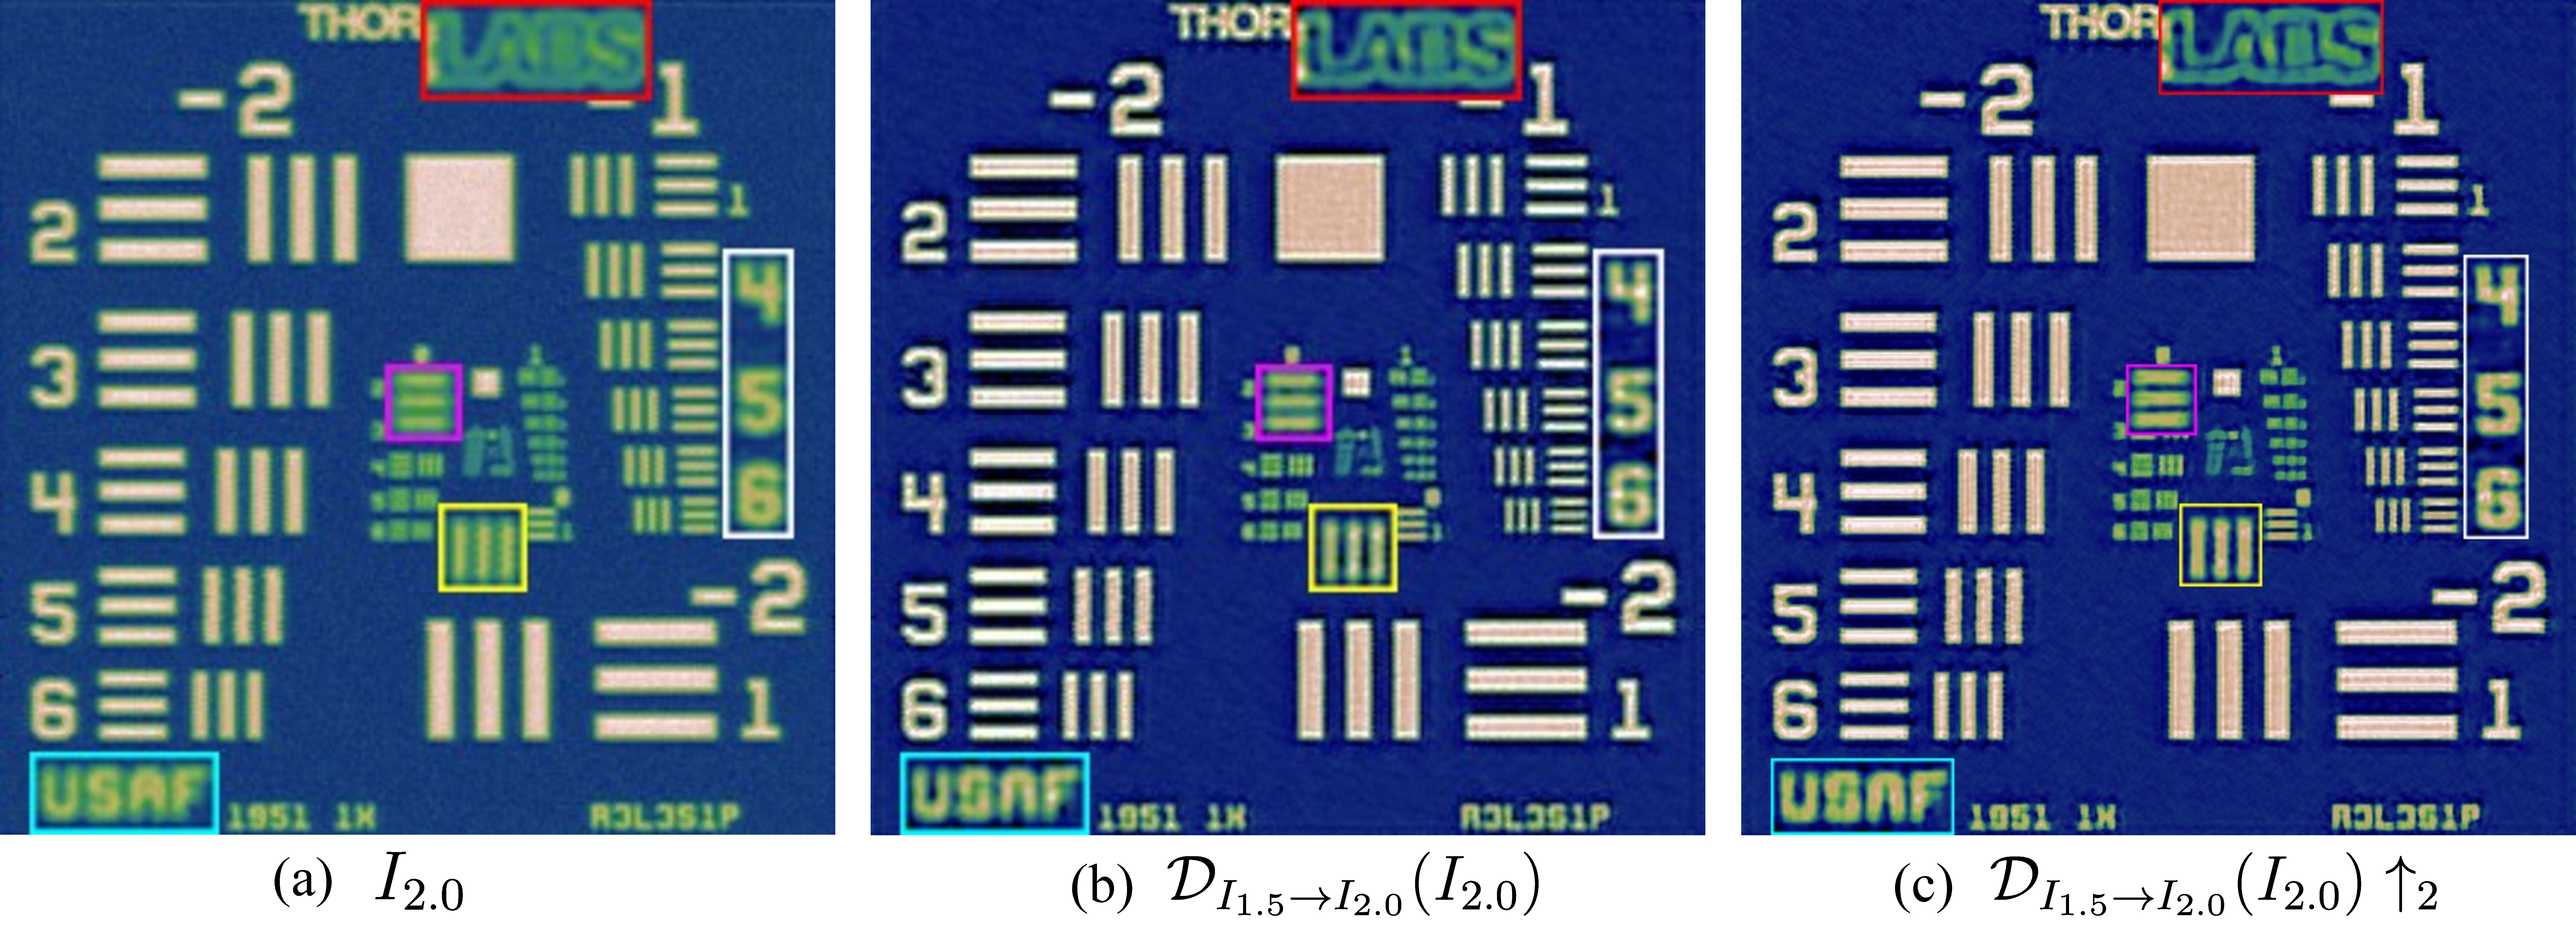
\includegraphics[width=\textwidth]{fig/Ryu-fig18.pdf}
    \caption{ZSSR results after applying O2O method. (a) Original 2.0 THz image; (b) O2O result ($\alpha=1.5,\beta=2.0,\gamma=2.0$); (c) ZSSR result of (b).}
    \label{fig:zssr}
\end{figure*}

\begin{figure*}[htbp]
    \centering
    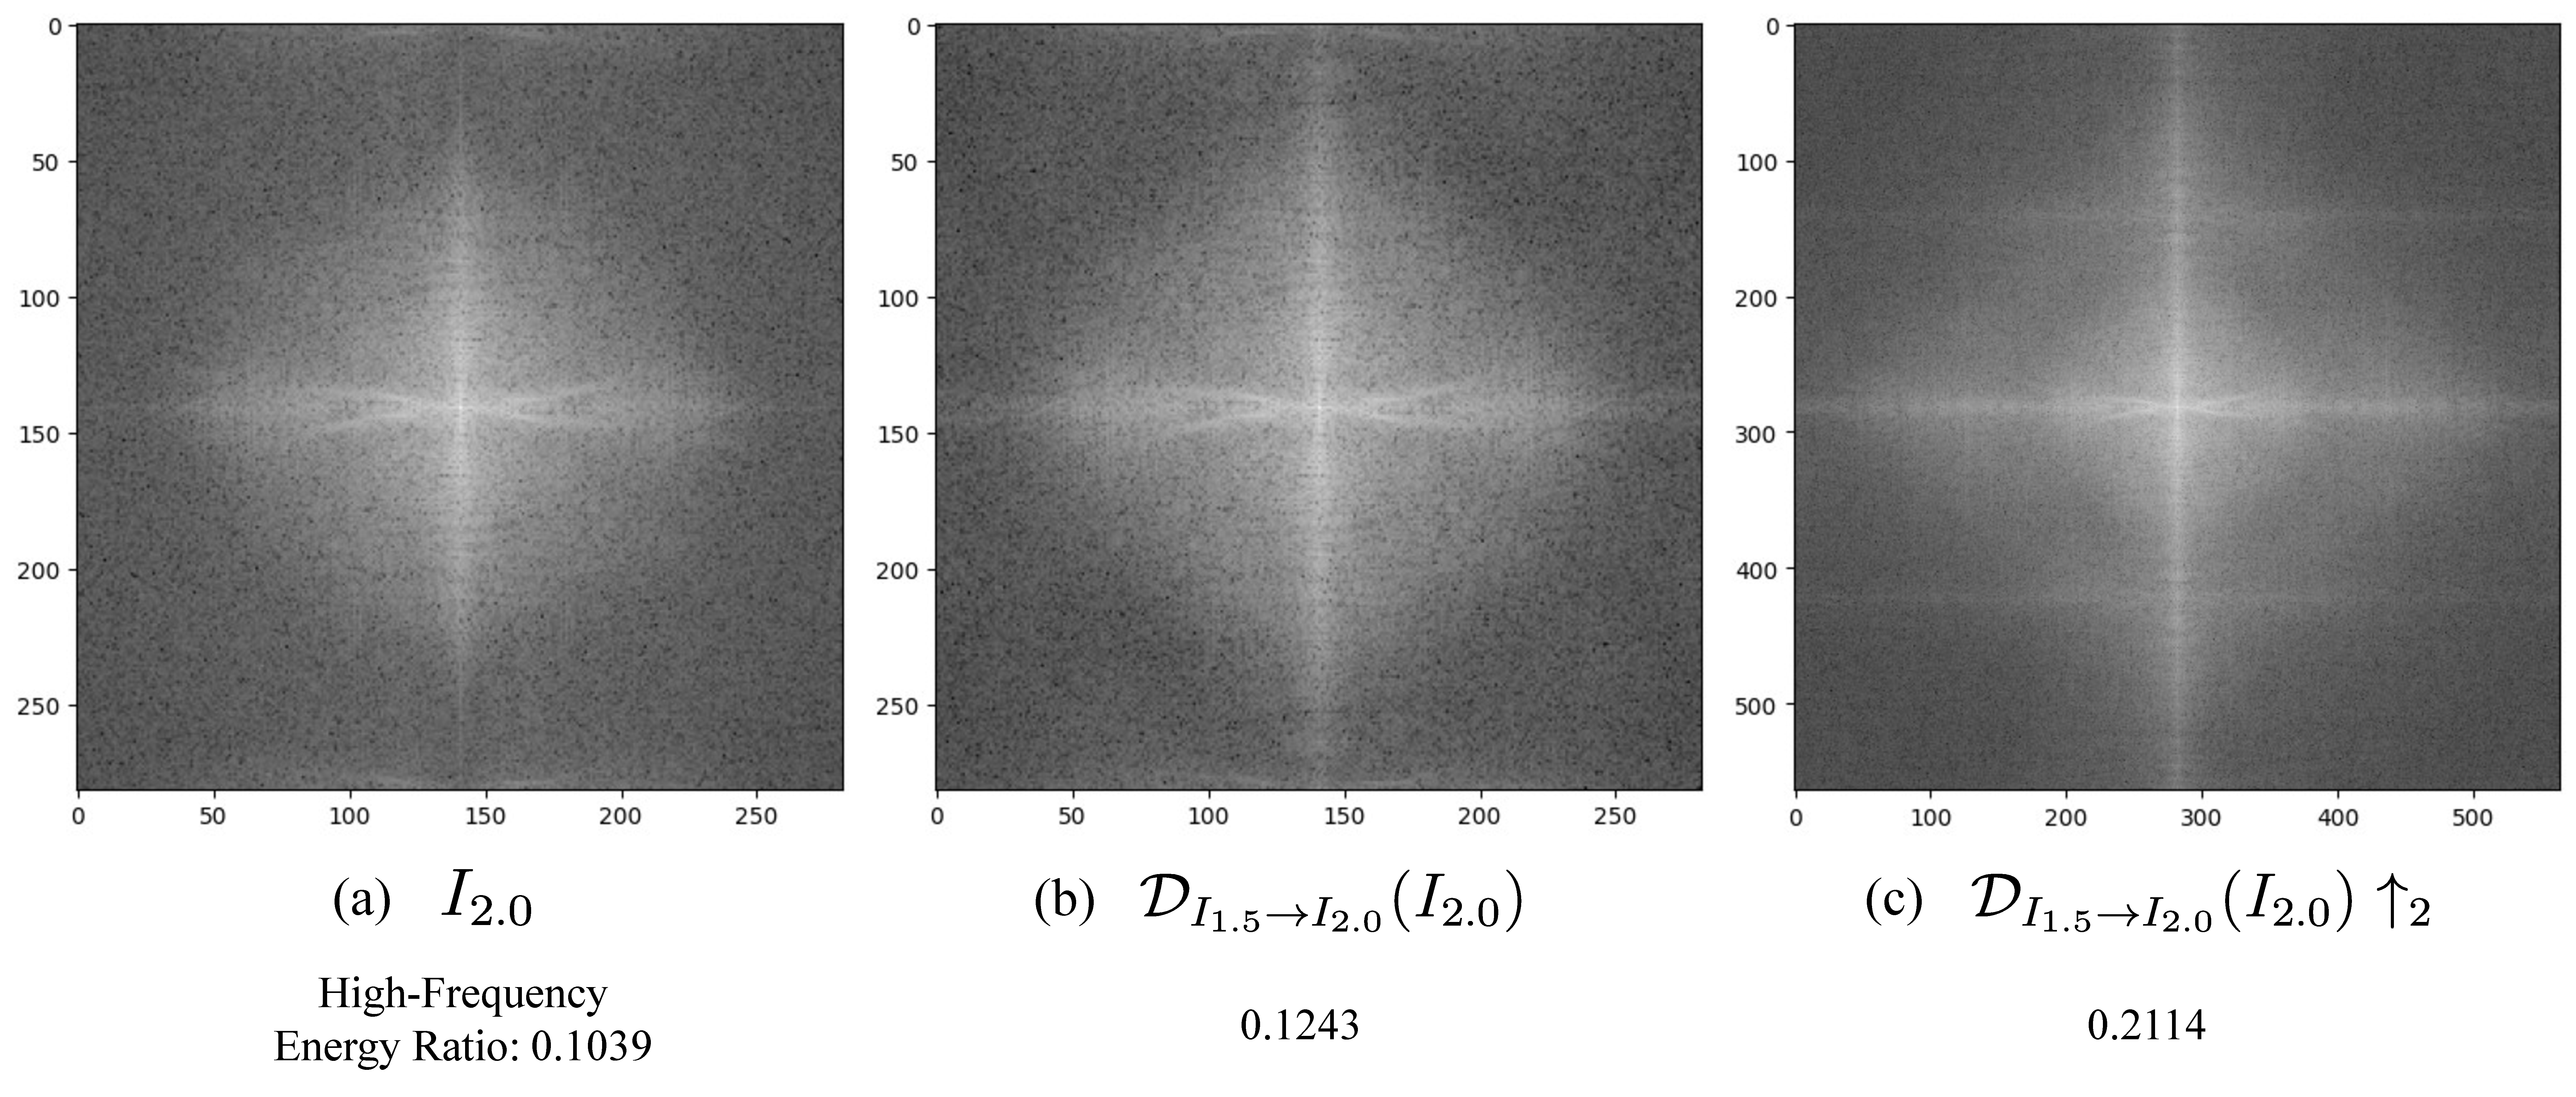
\includegraphics[width=0.95\textwidth]{fig/Ryu-fig19.pdf}
    \caption{Spatial frequency spectrum of ZSSR results.}
    \label{fig:zssr_spectrum}
\end{figure*}


%%% ---------- Subsection: Model Comparison ---------- %%%
\subsection{Model Comparison}
To demonstrate the efficacy of the proposed THz image-restoration method, we compared it with other deep learning-based image restoration methods, as shown in Fig.~\ref{fig:model-comp}. For a unbiased comparison, we applied a 2x resolution-enhancement process to all the other image-restoration methods, similar to our proposed learning method. The original 2.0 THz image has 282$\times$282 pixels, while the other results all have a resolution doubled to 584$\times$584 pixels. Consequently, except for the original image, all inferred images indicated a 2x increase in resolution, which resulted in a relative decrease in sharpness compared with the original image owing to the increased total number of pixels. Therefore, when evaluating the sharpness performance of the inferred images, one should compare the sharpness of the images excluding that of the original image.
Fig.~\ref{fig:model-comp}a shows the original 2.0 THz image. Figs.~\ref{fig:model-comp}b, c, and d show the images with twice the resolutions in the horizontal and vertical directions, which were achieved using networks proposed by Long et al.~\cite{longTerahertzImageSuperresolution2019}, HAN~\cite{niu2020han}, and NAFNetSR~\cite{chu2022nafssr}, respectively. Long et al.~\cite{longTerahertzImageSuperresolution2019} adopted a residual learning network structure, trained using a random degradation model. Figs.~\ref{fig:model-comp}c and d for HAN and NAFNetSR, represent state-of-the-art models in image SR. which were trained using the DIV2K dataset and degraded randomly using blur kernel widths measuring between 0.1 and 3~\cite{longTerahertzImageSuperresolution2019}.
Fig.~\ref{fig:model-comp}e shows the result of blur removal using pretrained NAFNet~\cite{chen2022simple} weights and by applying ZSSR. Fig.~\ref{fig:model-comp}f shows the results of training and inference using a combination of self-supervised learning on THz SAHS images and ZSSR, as proposed in this study. The ZSSR-applied images presented in Figs.~\ref{fig:model-comp}e and f appeared sharper and performed better numerically. In particular, in the yellow box, the edges became sharper and the boundaries were more clearly distinguished. In Figs.~\ref{fig:model-comp}b-\ref{fig:model-comp}d, where artificial Gaussian blur was applied and then restored, the edges became rounded and were smudged. This is because the artificial degradation implemented during the training was not optimized for the characteristics of the actual THz images. Based on Fig.~\ref{fig:model-comp}e, distortion in the form of a new blurred pattern in the background occurred owing to the addition of ZSSR after NAFNet, thus indicating that NAFNet and ZSSR did not integrate organically. As shown in Fig.~\ref{fig:model-comp}f, our proposed method yielded the highest sharpness and contrast, both visually and numerically. This is because our proposed method applies an image restoration method using pure frequency characteristics without artificial manipulation, utilizes THz SAHS images for self-supervised learning, and effectively combines image restoration with SR by integrating ZSSR into the self-supervised learning process.

\begin{figure*}[htbp]
    \centering
    \includegraphics[width=0.9\textwidth]{fig/Ryu-fig20.pdf}
    \caption{Performance comparison of deep THz image restoration methods. (a) Original 2.0 THz image; (b) results of Long et al.~\cite{longTerahertzImageSuperresolution2019}; (c) HAN~\cite{niu2020han}; (d) NAFNetSR~\cite{chu2022nafssr}; (e) NAFNet~\cite{chen2022simple}+ZSSR; (f) our results.}
    \label{fig:model-comp}
\end{figure*}